%%%%%%%%%%%%%%%%%%%%%%%%%%%%%%%%%%%%%%%%%
% Classicthesis Typographic Thesis
% LaTeX Template
% Version 1.4 (1/1/16)
%
% This template has been downloaded from:
% http://www.LaTeXTemplates.com
%
% Original author:
% André Miede (http://www.miede.de) with commenting modifications by:
% Vel (vel@LaTeXTemplates.com)
%
% License:
% GNU General Public License (v2)
%
% General Tips:
% 1) Make sure to edit the classicthesis-config.file
% 2) New enumeration (A., B., C., etc in small caps): \begin{aenumerate} \end{aenumerate}
% 3) For margin notes: \marginpar or \graffito{}
% 4) Do not use bold fonts in this style, it is designed around them
% 5) Use tables as in the examples
% 6) See classicthesis-preamble.sty for useful commands
%
%%%%%%%%%%%%%%%%%%%%%%%%%%%%%%%%%%%%%%%%%

%----------------------------------------------------------------------------------------
%	PACKAGES AND OTHER DOCUMENT CONFIGURATIONS
%----------------------------------------------------------------------------------------

\documentclass[
		twoside,openright,titlepage,numbers=noenddot,headinclude,%1headlines,
	 	footinclude=true,cleardoublepage=empty,
		dottedtoc, % Make page numbers in the table of contents flushed right with dots leading to them
		BCOR=5mm,paper=a4,fontsize=11pt, % Binding correction, paper type and font size
		ngerman,dutch, % Languages, change this to your language(s)
		]{scrreprt}

% Includes the file which contains all the document configurations and packages - make sure to edit this file
%%%%%%%%%%%%%%%%%%%%%%%%%%%%%%%%%%%%%%%%%
% Classicthesis Typographic Thesis
% Configuration File
%
% This file has been downloaded from:
% http://www.LaTeXTemplates.com
%
% Original author:
% André Miede (http://www.miede.de) with extensive commenting changes by:
% Vel (vel@LaTeXTemplates.com)
%
% License:
% GNU General Public License (v2)
%
% Important note:
% The main lines to change in this file are in the DOCUMENT VARIABLES
% section, the rest of the file is for advanced configuration.
%
%%%%%%%%%%%%%%%%%%%%%%%%%%%%%%%%%%%%%%%%%

%----------------------------------------------------------------------------------------
%	CHARACTER ENCODING
%----------------------------------------------------------------------------------------

\PassOptionsToPackage{utf8}{inputenc} % Set the encoding of your files. UTF-8 is the only sensible encoding nowadays. If you can't read äöüßáéçèê∂åëæƒÏ€ then change the encoding setting in your editor, not the line below. If your editor does not support utf8 use another editor!
\usepackage{inputenc}

%----------------------------------------------------------------------------------------
%	DOCUMENT VARIABLES
%	Fill in the lines below to enter your information into the thesis template
%	Each of the commands can be cited anywhere in the thesis
%----------------------------------------------------------------------------------------

% Remove drafting to get rid of the '[ Date - classicthesis version 4.0 ]' text at the bottom of every page
%\PassOptionsToPackage{eulerchapternumbers,listings,drafting, pdfspacing, subfig,beramono,eulermath,parts}{classicthesis}
% Available options: drafting parts nochapters linedheaders eulerchapternumbers beramono eulermath pdfspacing minionprospacing tocaligned dottedtoc manychapters listings floatperchapter subfig

\newcommand{\myTitle}{Analysing SOUP\xspace}
\newcommand{\mySubtitle}{Een weg naar veiligere software\xspace}
\newcommand{\myDegree}{Doktor-Ingenieur (Dr.-Ing.)\xspace}
\newcommand{\myName}{Bas Brunink\xspace}
\newcommand{\myFaculty}{FDMCI\xspace}
\newcommand{\myDepartment}{Software Engineering\xspace}
\newcommand{\myUni}{Hogeschool van Amsterdam\xspace}
\newcommand{\myHvABegeleider}{Fatih Caglayan}
\newcommand{\myLocation}{Amsterdam\xspace}
\newcommand{\myTime}{Februari 2022\xspace}
\newcommand{\myVersion}{version 1\xspace}

\newcommand{\myStagebegeleider}{Bas Breijer \xspace}
\newcommand{\myworkName}{Eaglescience\xspace}
\newcommand{\myworkAddress}{Naritaweg 12K\xspace}
\newcommand{\myworkPostcodeCity}{1043 BZ Amsterdam\xspace}


%----------------------------------------------------------------------------------------
%	USEFUL COMMANDS
%----------------------------------------------------------------------------------------

\newcommand{\ie}{i.\,e.}
\newcommand{\Ie}{I.\,e.}
\newcommand{\eg}{e.\,g.}
\newcommand{\Eg}{E.\,g.}

\newcounter{dummy} % Necessary for correct hyperlinks (to index, bib, etc.)
\providecommand{\mLyX}{L\kern-.1667em\lower.25em\hbox{Y}\kern-.125emX\@}
\newlength{\abcd} % for ab..z string length calculation

%----------------------------------------------------------------------------------------
%	PACKAGES
%----------------------------------------------------------------------------------------

\usepackage{lipsum} % Used for inserting dummy 'Lorem ipsum' text into the template

%------------------------------------------------

%\PassOptionsToPackage{ngerman,american}{babel}  % Change this to your language(s)
% Spanish languages need extra options in order to work with this template
%\PassOptionsToPackage{spanish,es-lcroman}{babel}
\usepackage{babel}

%------------------------------------------------

\usepackage{csquotes}
\PassOptionsToPackage{%
%backend=biber, % Instead of bibtex
backend=bibtex8,bibencoding=ascii,%
language=auto,%
%style=numeric-comp,%
style=authoryear-comp, % Author 1999, 2010
%bibstyle=authoryear,dashed=false, % dashed: substitute rep. author with ---
sorting=nyt, % name, year, title
maxbibnames=10, % default: 3, et al.
%backref=true,%
natbib=true % natbib compatibility mode (\citep and \citet still work)
}{biblatex}
\usepackage{biblatex}

 %------------------------------------------------

\PassOptionsToPackage{fleqn}{amsmath} % Math environments and more by the AMS
 \usepackage{amsmath}

 %------------------------------------------------

\PassOptionsToPackage{T1}{fontenc} % T2A for cyrillics
\usepackage{fontenc}

%------------------------------------------------

\usepackage{textcomp} % Fix warning with missing font shapes

%------------------------------------------------

\usepackage{scrhack} % Fix warnings when using KOMA with listings package

%------------------------------------------------

\usepackage{xspace} % To get the spacing after macros right

%------------------------------------------------

\usepackage{mparhack} % To get marginpar right

%------------------------------------------------

%\usepackage{fixltx2e} % Fixes some LaTeX stuff

%------------------------------------------------

\usepackage{url} %% fix for urls in cites

\PassOptionsToPackage{smaller}{acronym} % Include printonlyused in the first bracket to only show acronyms used in the text
\usepackage{acronym} % Nice macros for handling all acronyms in the thesis

%\renewcommand*{\acsfont}[1]{\textssc{#1}} % For MinionPro
\renewcommand*{\aclabelfont}[1]{\acsfont{#1}}

%------------------------------------------------

\PassOptionsToPackage{pdftex}{graphicx}
\usepackage{graphicx}

%----------------------------------------------------------------------------------------
%	FLOATS: TABLES, FIGURES AND CAPTIONS SETUP
%----------------------------------------------------------------------------------------

\usepackage{tabularx} % Better tables
\setlength{\extrarowheight}{3pt} % Increase table row height
\newcommand{\tableheadline}[1]{\multicolumn{1}{c}{\spacedlowsmallcaps{#1}}}
\newcommand{\myfloatalign}{\centering} % To be used with each float for alignment
\usepackage{caption}
\captionsetup{font=small}
\usepackage{subfig}

%----------------------------------------------------------------------------------------
%	CODE LISTINGS SETUP
%----------------------------------------------------------------------------------------

\usepackage{listings}
%\lstset{emph={trueIndex,root},emphstyle=\color{BlueViolet}}%\underbar} % For special keywords
\lstset{language=[LaTeX]Tex,%C++ % Specify the language(s) for listings here
morekeywords={PassOptionsToPackage,selectlanguage},
keywordstyle=\color{RoyalBlue}, % Add \bfseries for bold
basicstyle=\small\ttfamily, % Makes listings a smaller font size and a different font
%identifierstyle=\color{NavyBlue}, % Color of text inside brackets
commentstyle=\color{Green}\ttfamily, % Color of comments
stringstyle=\rmfamily, % Font type to use for strings
numbers=left, % Change left to none to remove line numbers
numberstyle=\scriptsize, % Font size of the line numbers
stepnumber=5, % Increment of line numbers
numbersep=8pt, % Distance of line numbers from code listing
showstringspaces=false, % Sets whether spaces in strings should appear underlined
breaklines=true, % Force the code to stay in the confines of the listing box
%frameround=ftff, % Uncomment for rounded frame
%frame=single, % Frame border - none/leftline/topline/bottomline/lines/single/shadowbox/L
belowcaptionskip=.75\baselineskip % Space after the "Listing #: Desciption" text and the listing box
}

%----------------------------------------------------------------------------------------
%	HYPERREFERENCES
%----------------------------------------------------------------------------------------

\PassOptionsToPackage{pdftex,hyperfootnotes=false,pdfpagelabels}{hyperref}
\usepackage{hyperref}  % backref linktocpage pagebackref
\pdfcompresslevel=9
\pdfadjustspacing=1

\hypersetup{
% Uncomment the line below to remove all links (to references, figures, tables, etc), useful for b/w printouts
%draft,
colorlinks=true, linktocpage=true, pdfstartpage=3, pdfstartview=FitV,
% Uncomment the line below if you want to have black links (e.g. for printing black and white)
%colorlinks=false, linktocpage=false, pdfborder={0 0 0}, pdfstartpage=3, pdfstartview=FitV,
breaklinks=true, pdfpagemode=UseNone, pageanchor=true, pdfpagemode=UseOutlines,%
plainpages=false, bookmarksnumbered, bookmarksopen=true, bookmarksopenlevel=1,%
hypertexnames=true, pdfhighlight=/O,%nesting=true,%frenchlinks,%
urlcolor=webbrown, linkcolor=RoyalBlue, citecolor=webgreen, %pagecolor=RoyalBlue,%
    %urlcolor=Black, linkcolor=Black, citecolor=Black, %pagecolor=Black,%
%------------------------------------------------
% PDF file meta-information
pdftitle={\myTitle},
pdfauthor={\textcopyright\ \myName, \myUni, \myFaculty},
pdfsubject={},
pdfkeywords={},
pdfcreator={pdfLaTeX},
pdfproducer={LaTeX with hyperref and classicthesis}
%------------------------------------------------
}

%----------------------------------------------------------------------------------------
%	AUTOREFERENCES SETUP
%	Redefines how references in text are prefaced for different
%	languages (e.g. "Section 1.2" or "section 1.2")
%----------------------------------------------------------------------------------------

\makeatletter
\@ifpackageloaded{babel}
{
\addto\extrasamerican{
\renewcommand*{\figureautorefname}{Figure}
\renewcommand*{\tableautorefname}{Table}
\renewcommand*{\partautorefname}{Part}
\renewcommand*{\chapterautorefname}{Chapter}
\renewcommand*{\sectionautorefname}{Section}
\renewcommand*{\subsectionautorefname}{Section}
\renewcommand*{\subsubsectionautorefname}{Section}
}
\addto\extrasngerman{
\renewcommand*{\paragraphautorefname}{Absatz}
\renewcommand*{\subparagraphautorefname}{Unterabsatz}
\renewcommand*{\footnoteautorefname}{Fu\"snote}
\renewcommand*{\FancyVerbLineautorefname}{Zeile}
\renewcommand*{\theoremautorefname}{Theorem}
\renewcommand*{\appendixautorefname}{Anhang}
\renewcommand*{\equationautorefname}{Gleichung}
\renewcommand*{\itemautorefname}{Punkt}
}
\providecommand{\subfigureautorefname}{\figureautorefname} % Fix to getting autorefs for subfigures right
}{\relax}
\makeatother

%----------------------------------------------------------------------------------------
%\usepackage[apaciteclassic, notocbib, nodoi, nosectionbib]{apacite}


\usepackage{classicthesis}

%----------------------------------------------------------------------------------------
%	CHANGING TEXT AREA
%----------------------------------------------------------------------------------------

\linespread{1.05} % a bit more for Palatino
\areaset[current]{445pt}{761pt} % 686 (factor 2.2) + 33 head + 42 head \the\footskip
%\setlength{\marginparwidth}{7em}%
%\setlength{\marginparsep}{2em}%

%----------------------------------------------------------------------------------------
%	USING DIFFERENT FONTS
%----------------------------------------------------------------------------------------

%\usepackage[oldstylenums]{kpfonts} % oldstyle notextcomp
%\usepackage[osf]{libertine}
%\usepackage[light,condensed,math]{iwona}
%\renewcommand{\sfdefault}{iwona}
%\usepackage{lmodern} % <-- no osf support :-(
%\usepackage{cfr-lm} %
%\usepackage[urw-garamond]{mathdesign} <-- no osf support :-(
%\usepackage[default,osfigures]{opensans} % scale=0.95
%\usepackage[sfdefault]{FiraSans}


\addbibresource{Bibliography.bib} % The file housing your bibliography
%\addbibresource[label=ownpubs]{Self_Publications.bib} % Uncomment for optional self-publications

%\hyphenation{Put special hyphenation here}

\begin{document}

\frenchspacing % Reduces space after periods to make text more compact

\raggedbottom % Makes all pages the height of the text on that page

\selectlanguage{dutch} % Select your default language - e.g. american or ngerman

%\renewcommand*{\bibname}{new name} % Uncomment to change the name of the bibliography
%\setbibpreamble{} % Uncomment to include a preamble to the bibliography - some text before the reference list starts

\pagenumbering{roman} % Roman page numbering prior to the start of the thesis content (i, ii, iii, etc)

\pagestyle{plain} % Suppress headers for the pre-content pages

%----------------------------------------------------------------------------------------
%	PRE-CONTENT THESIS PAGES
%----------------------------------------------------------------------------------------

% Title Page

\begin{titlepage}

    \begin{addmargin}[-1cm]{-3cm}
        \begin{center}
            \large

            \hfill
            \vfill

            \begingroup
            {\color[HTML]{27406B}\spacedallcaps {\Huge\myTitle} \\ \bigskip} % Thesis title
            {\color[HTML]{84C6C8}\Large\mySubtitle \\ \medskip}

            \endgroup
            \spacedlowsmallcaps{\large\myName} % Your name

            \vfill

            %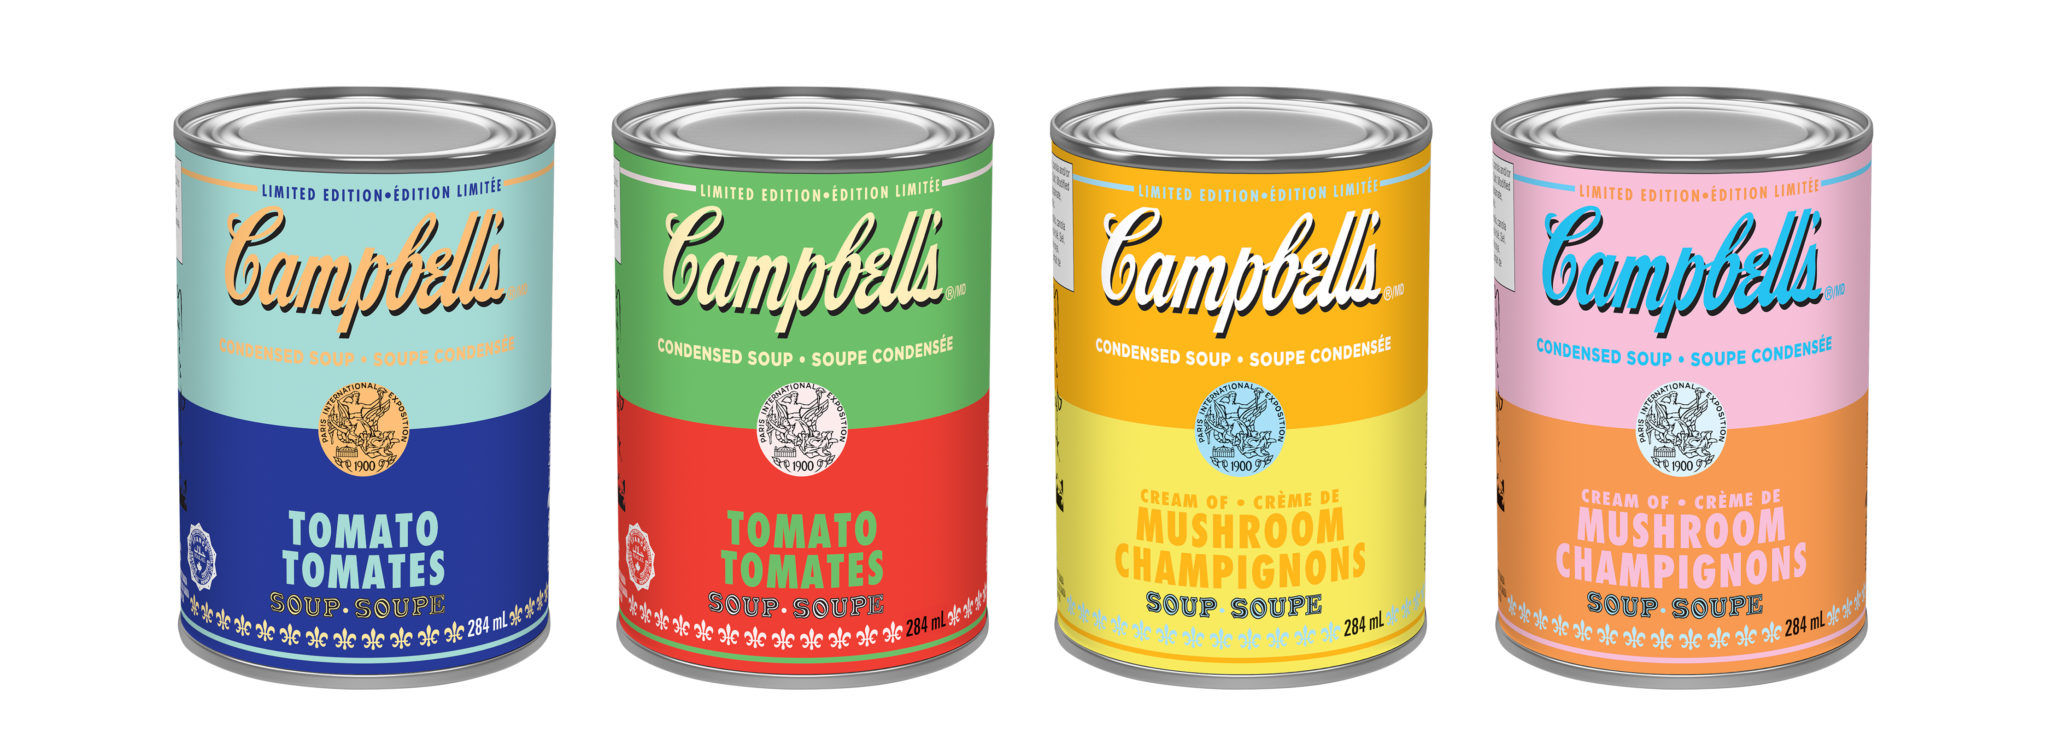
\includegraphics[width=15cm]{gfx/soupcans} \\  % Picture
            
\includegraphics[width=15cm]{gfx/EagleScience_Logo_on_white} \\  % Picture
            % Thesis subtitle
            % %\myDegree \\


            Begeleiding:\\ \bigskip
            EagleScience\\
            \myStagebegeleider \\
            \medskip
            Hogeschool van Amsterdam\\
            \myHvABegeleider \\ \bigskip \bigskip \bigskip


            \myTime % Time and version

            \vfill

        \end{center}
    \end{addmargin}

\end{titlepage}
 % Main title page

% Back of the title page

\thispagestyle{empty}

\hfill

\vfill

\noindent\myName: \textit{\myTitle,} \mySubtitle, %\myDegree, 
\textcopyright\ \myTime

% You may wish to do something with the back of the title page, such as including your supervisors, location or time frame of the work. Below is an example of doing so although you may want to tweak it to your liking.

%\bigskip

%\noindent\spacedlowsmallcaps{Supervisors}: \\
%\myProf \\
%\myOtherProf \\ 
%\mySupervisor

%\medskip \\

%\noindent\spacedlowsmallcaps{Location}: \\
%\myLocation

%\medskip \\

%\noindent\spacedlowsmallcaps{Time Frame}: \\
%\myTime
 % Back of the title page

%\cleardoublepage% Dedication

\thispagestyle{empty}
\refstepcounter{dummy}

\pdfbookmark[1]{Dedication}{Dedication} % Bookmark name visible in a PDF viewer

\vspace*{3cm}

\begin{center}
\emph{Ohana} means family. \\
Family means nobody gets left behind, or forgotten. \\ \medskip
--- Lilo \& Stitch    
\end{center}

\medskip

\begin{center}
Dedicated to the loving memory of Rudolf Miede. \\ \smallskip
1939\,--\,2005
\end{center} % Dedication page

\cleardoublepage\chapter{Inleiding}\label{ch:inleiding}
Dit afstudeerverslag is het resultaat van de afstudeeropdracht welke is uitgevoerd in opdracht voor het bedrijf Eaglescience. Sinds 2009 richt Eaglescience zich op de ontwikkeling van complexe software oplossingen voor haar klanten op projectbasis.

Eaglescience hecht belang aan de ontwikkeling van zo veilig mogelijke software oplossingen voor haar klanten. Tijdens de ontwikkeling van applicaties maakt Eaglescience gebruik van externe bibliotheken, waardoor kwetsbaarheden in applicaties zouden kunnen worden geïntroduceerd. Eén van de manieren om software veiliger te maken is door het uitvoeren van ‘Software of Unknown Provenance’ analyses, ook wel SOUP-analyses genoemd. Deze analyses maken kwetsbaarheden in externe software inzichtelijk, zodat hierop actie kan worden ondernomen. Groei binnen Eaglescience en de hierdoor steeds groter wordende variabiliteit aan applicaties heeft ertoe geleidt dat er behoefte is ontstaan om SOUP-analyses op een geautomatiseerde manier op periodieke basis uit te voeren. De centrale onderzoeksvraag van deze afstudeeropdracht luidt; ‘Hoe kan Eaglescience middels een geautomatiseerde methode inzicht krijgen in potentiële kwetsbaarheden van gebruikte bibliotheken binnen projecten, waarbij rekening gehouden wordt met de huidige manier van werken?’.

De afstudeeropdracht is een aantal fasen uitgevoerd welke ieders in een eigen deel worden beschreven:
Deel~\ref{prt:opdracht} beschrijft het onderzoek naar Eaglescience zelf, hun werkwijze en de opdracht voor het afstudeerproject. In deel~\ref{prt:Onderzoek} wordt het onderzoeksplan besproken waarin middels een probleemanalyse, stakeholdersanalyse, en een conceptueel model naar een onderzoeksvraag met daaruit volgende deelvragen wordt gewerkt die vervolgens worden uitgewerkt en onderzocht. Het onderzoek zelf is ingedeeld in een theoretisch hoofdstuk waarin wordt onderzocht welke rol Software of Unkown provenance heeft in het ontwikkelen van software, welke gevaren het gebruik hiervan met zich mee kan brengen alsook welke instellingen zich bezig houden met het vastleggen van deze gevaren. Vervolgens wordt er gezocht naar tooling en een methode die binnen Eaglescience gebruikt kan worden om te achterhalen of er zich daadwerkelijk gevaren bevinden in de door Eaglescience ontwikkelde software. De uitkomst van dit laatste onderzoek is de basis voor het ontwerp van een applicatie welke in deel~\ref{prt:ontwerp} is beschreven. In dit deel wordt het ontwerp van de applicatie beschreven beginnend met de architectuur om vervolgens een aantal belangrijke onderdelen functioneel toe te lichten. Het afstudeerverslag wordt afgesloten door  deel~\ref{prt:conclusie}, waarin de eindconclusie wordt gegeven.


 % Uncomment and create a Foreword.tex to include a foreword

\cleardoublepage% Abstract

%\renewcommand{\abstractname}{Abstract} % Uncomment to change the name of the abstract

\pdfbookmark[1]{Samenvatting}{Samenvatting} % Bookmark name visible in a PDF viewer

\chapter{Samenvatting}\label{ch:samenvatting}

De in dit afstudeerverslag beschreven afstudeeropdracht is uitgevoerd in opdracht van Eaglescience, een bedrijf welke software op maat ontwikkeld voor een grote verscheidenheid aan klanten. Tijdens de ontwikkeling van software maakt Eaglescience gebruik van externe bibliotheken. Door het gebruik hiervan zouden er echter potentiele gevaren kunnen worden geintroduceerd in de software. Om deze gevaren inzichtelijk te maken, zodat hierop actie kan worden ondernomen, zou Eaglescience een geautomatiseerde analyse methode willen inzetten. In dit afstudeerverslag worden de onderzoeken beschreven die zijn uitgevoerd met als doel om een applicatie te ontwerpen die geautomatiseerd en periodiek de kwetsbaarheden van externe bibliotheken, ofwel 'software of unknown provencance' (SOUP) in kaart kan brengen.
Tijdens het onderzoek zijn de eisen aan deze applicatie vanuit de opdrachtgever in kaart gebracht, en is er onderzocht welke tooling en methodiek het beste aansluit bij de huidige werkwijze, Dev-stack en tooling van Eaglescience. Het onderzoek wees uit dat Eaglescience werkt met Scala en TypeScript, waarbij SBT en NPM als buildtools worden gebruikt. Door ontwikkeling in deze niche-taal is de beschikbare tooling voor SOUP analyses gelimiteerd. De resultaten van het onderzoek gaven aan dat de OWASP-dependency-check (voor NPM) en de sbt-dependency-check (voor SBT) het beste kunnen worden gebruikt. Na het uitvoeren van een reeks testen met deze tooling bleek deze inderdaad geschikt te zijn voor de specifieke situatie van Eaglescience en te voldoen aan de eisen van de opdrachtgever. Op basis van de informatie komende uit deze onderzoeken is een ontwerp ontwikkeld voor een applicatie, welke geautmatiseerd en op periodieke basis SOUP analyses uit zou kunnen voeren. De ontworpen applicatie voldoet aan de eisen gesteld door de opdrachtgever en zou daarom binnen de huidige Dev-stack kunnen worden geimplementeerd.





\vfill
 % Abstract page

%\cleardoublepage% Publications - a page listing research articles written using content in the thesis

\pdfbookmark[1]{Publications}{Publications} % Bookmark name visible in a PDF viewer

\chapter*{Publications} % Publications page text

Some ideas and figures have appeared previously in the following publications:\\

\noindent Put your publications from the thesis here. The packages \texttt{multibib} or \texttt{bibtopic} etc. can be used to handle multiple different bibliographies in your document.

%\begin{refsection}[ownpubs]
%    \small
%    \nocite{*} % is local to to the enclosing refsection
%    \printbibliography[heading=none]
%\end{refsection}

%\emph{Attention}: This requires a separate run of \texttt{bibtex} for your \texttt{refsection}, \eg, \texttt{ClassicThesis1-blx} for this file. You might also use \texttt{biber} as the backend for \texttt{biblatex}. See also \url{http://tex.stackexchange.com/questions/128196/problem-with-refsection}. % Publications from the thesis page

%\cleardoublepage% Acknowledgements

\pdfbookmark[1]{Acknowledgements}{Acknowledgements} % Bookmark name visible in a PDF viewer

\begin{flushright}{\slshape    
We have seen that computer programming is an art, \\ 
because it applies accumulated knowledge to the world, \\ 
because it requires skill and ingenuity, and especially \\
because it produces objects of beauty.} \\ \medskip
--- \defcitealias{knuth:1974}{Donald E. Knuth}\citetalias{knuth:1974} \citep{knuth:1974}
\end{flushright}

\bigskip

%----------------------------------------------------------------------------------------

\begingroup

\let\clearpage\relax
\let\cleardoublepage\relax
\let\cleardoublepage\relax

\chapter*{Acknowledgements}

\noindent Put your acknowledgements here.\\

\noindent Many thanks to everybody who already sent me a postcard!\\

\noindent Regarding the typography and other help, many thanks go to Marco Kuhlmann, Philipp Lehman, Lothar Schlesier, Jim Young, Lorenzo Pantieri and Enrico Gregorio\footnote{Members of GuIT (Gruppo Italiano Utilizzatori di \TeX\ e \LaTeX )}, J\"org Sommer, Joachim K\"ostler, Daniel Gottschlag, Denis Aydin, Paride Legovini, Steffen Prochnow, Nicolas Repp, Hinrich Harms, Roland Winkler, and the whole \LaTeX-community for support, ideas and some great software.

\bigskip

\noindent\emph{Regarding \mLyX}: The \mLyX\ port was initially done by
\emph{Nicholas Mariette} in March 2009 and continued by
\emph{Ivo Pletikosi\'c} in 2011. Thank you very much for your work and the contributions to the original style.

\endgroup % Acknowledgements page

\pagestyle{scrheadings} % Show chapter titles as headings

\cleardoublepage% Table of Contents - List of Tables/Figures/Listings and Acronyms

\refstepcounter{dummy}

\pdfbookmark[1]{\contentsname}{tableofcontents} % Bookmark name visible in a PDF viewer

\setcounter{tocdepth}{2} % Depth of sections to include in the table of contents - currently up to subsections

\setcounter{secnumdepth}{3} % Depth of sections to number in the text itself - currently up to subsubsections

\manualmark
\markboth{\spacedlowsmallcaps{\contentsname}}{\spacedlowsmallcaps{\contentsname}}
\tableofcontents
\automark[section]{chapter}
\renewcommand{\chaptermark}[1]{\markboth{\spacedlowsmallcaps{#1}}{\spacedlowsmallcaps{#1}}}
\renewcommand{\sectionmark}[1]{\markright{\thesection\enspace\spacedlowsmallcaps{#1}}}

\clearpage

\begingroup
\let\clearpage\relax
\let\cleardoublepage\relax
\let\cleardoublepage\relax

%----------------------------------------------------------------------------------------
%	List of Figures
%----------------------------------------------------------------------------------------

\refstepcounter{dummy}
%\addcontentsline{toc}{chapter}{\listfigurename} % Uncomment if you would like the list of figures to appear in the table of contents
\pdfbookmark[1]{\listfigurename}{lof} % Bookmark name visible in a PDF viewer

\listoffigures

\vspace{8ex}
\newpage

%----------------------------------------------------------------------------------------
%	List of Tables
%----------------------------------------------------------------------------------------

\refstepcounter{dummy}
%\addcontentsline{toc}{chapter}{\listtablename} % Uncomment if you would like the list of tables to appear in the table of contents
\pdfbookmark[1]{\listtablename}{lot} % Bookmark name visible in a PDF viewer

\listoftables

\vspace{8ex}
\newpage

%----------------------------------------------------------------------------------------
%	List of Listings
%----------------------------------------------------------------------------------------

\refstepcounter{dummy}
%\addcontentsline{toc}{chapter}{\lstlistlistingname} % Uncomment if you would like the list of listings to appear in the table of contents
\pdfbookmark[1]{\lstlistlistingname}{lol} % Bookmark name visible in a PDF viewer

\lstlistoflistings

\vspace{8ex}
\newpage

%----------------------------------------------------------------------------------------
%	Acronyms
%----------------------------------------------------------------------------------------

\refstepcounter{dummy}
%\addcontentsline{toc}{chapter}{Acronyms} % Uncomment if you would like the acronyms to appear in the table of contents
\pdfbookmark[1]{Acronyms}{acronyms} % Bookmark name visible in a PDF viewer

\markboth{\spacedlowsmallcaps{Acronyms}}{\spacedlowsmallcaps{Acronyms}}

\chapter*{Acroniemen}

\begin{acronym}[UML]
\acro{DRY}{Don't Repeat Yourself}
\acro{API}{Application Programming Interface}
\acro{UML}{Unified Modeling Language}
\end{acronym}

\endgroup
 % Contents, list of figures/tables/listings and acronyms

\cleardoublepage

\pagenumbering{arabic} % Arabic page numbering for thesis content (1, 2, 3, etc)
%\setcounter{page}{90} % Uncomment to manually start the page counter at an arbitrary value (for example if you wish to count the pre-content pages in the page count)

\cleardoublepage % Avoids problems with pdfbookmark

%----------------------------------------------------------------------------------------
%	THESIS CONTENT - CHAPTERS
%----------------------------------------------------------------------------------------


\part{Opdracht}\label{prt:opdracht}

% Chapter 1
\chapter{Eaglescience}\label{ch:Eaglescience} % Chapter title

Het hier beschreven onderzoek en het daarbij behorende ontwerp voor een applicatie is uitgevoerd en ontwikkeld in opdracht van het bedrijf Eaglescience. Dit bedrijf is gevestigd in Amsterdam Sloterdijk en houdt zich sinds 2009 bezig met het ontwikkelen van software. Hoewel het ontwikkelen van maatwerk software de kern activiteit is biedt het bedrijf ook een aantal andere diensten aan, zoals het bouwen van prototypes of het meedenken in een design sprint om bedrijven en startups een goede richting te geven voor het ontwikkelen van een project. Daarnaast biedt Eaglescience hosting aan voor de software die door hun is ontwikkeld, om zo garantie te kunnen bieden dat er alles aan wordt gedaan zodat de geleverde software veilig, kwalitatief goed en correct functioneert.

\section{Organisatie}\label{sec:organisatie}
Eaglescience BV bestaat uit drie divisies: Innovations, Software en Solutions (figuur~\ref{fig:Eaglescience organogram}). Er werken, op het moment van schrijven, $\pm$ 20 medewerkers waarvan 75\% verantwoordelijk is voor de ontwikkeling van software. De andere 25\% bekleed een support rol zoals project manager, finance manager, quality manager, automatisering etc.

\begin{figure}[bth]
\myfloatalign
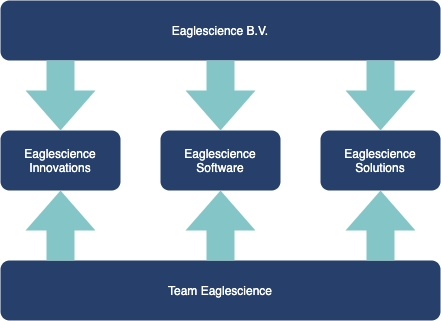
\includegraphics[width=9cm]{gfx/organogram}
\caption{Organogram Eaglescience}
\label{fig:Eaglescience organogram}
\end{figure}
De divisie Eaglescience Innovations zoekt naar nieuwe oplossingen op het gebied van softwareontwikkeling, welke door de divisie Eaglescience Software wordt geïmplementeerd. Eaglescience Solutions onderzoekt en adviseert over oplossingen voor gestelde problemen. Onder het dagelijks bestuur valt Team Eaglescience dat bestaat uit projectmanagers en ontwikkelaars. Deze zijn onderverdeeld in diverse scrum teams die ieder verantwoordelijk zijn voor een project. De ontwikkelaars worden parallel ingezet op meerdere projecten om kennisdeling te bevorderen.

\subsection{Missie}\label{subsec:missie}

De missie van Eaglescience is het bedienen van haar partners door een ontwerp, ontwikkeling en service te bieden op het gebied van op maat gemaakte IT-oplossingen. Hiervoor heeft Eaglescience goed opgeleide IT-professionals in dienst die zichzelf continue ontwikkelen op de “cutting edge” van IT-technologie. De hoofdcompetenties van de medewerkers zijn: innovatief, intelligent, klant georiënteerd, flexibel en ambitieus~\citep{Eaglescience:2020}.

\subsection{Visie}\label{subsec:visie}
Eaglescience streeft er als innovatief IT-bedrijf naar om software te ontwikkelen als een Business-to-Business dienst. Middels technische vaardigheden bouwen we veilige en hoogwaardige software die bijdraagt aan een betere wereld. Omdat we Agile werken, leveren we precies wat nodig is, niets meer en niets minder. Wij helpen onze klanten zoeken naar een langdurige betrokkenheid en samenwerking op basis van zowel vertrouwen als wederzijds respect.

Omdat elke vraag uniek is, ontwikkeld Eaglescience op maat gemaakte en innovatieve software.  We zijn van plan deel uit te maken van het hele proces van het formuleren van een idee tot het lanceren van het product en het waarborgen van de productie levenscyclus. Onze belangrijkste succesfactor zijn de mensen, die zich continu ontwikkelen door met de nieuwste technieken te werken op diverse projecten. Wij streven naar een optimale balans tussen werk en privé. Dit geeft onze medewerkers veel vrijheid, maar vereist zelfdiscipline en verantwoordelijkheid~\citep{Eaglescience:2020}.

\subsection{Strategie}\label{subsec:strategie}
Eaglescience levert de visie via vier strategische thema's:
\begin{itemize}
    \item Maatschappelijke verantwoordelijkheid
    \item Persoonlijke groei en werknemer tevredenheid
    \item Kwalitatief hoogstaande producten en diensten
    \item Financieël onafhankelijk en een sociaal verantwoorde groei
\end{itemize}
We streven er naar om veilige en hoogwaardige software diensten te leveren die waarde toevoegen aan onze samenleving. We streven naar een bedrijfscultuur waarin alle collega's hun talenten kunnen laten groeien. We hebben een ongecompliceerd werkethos: we richten ons op resultaten van hoge kwaliteit, maar met een gezonde balans tussen werk en privé en voldoende tijd voor leuke en sociale evenementen.
\newpage
Eaglescience verwacht van alle medewerkers dat zij hun handelen baseren op vier kwaliteitsprincipes:
\begin{itemize}
    \item Meld situaties die niet voldoen aan onze interne procedures
    \item Evalueer risico's wanneer grote veranderingen worden verwacht
    \item Help en daag elkaar uit
    \item Kennis behouden over conformiteit en kwaliteitsmanagement
\end{itemize}

\section{Werkwijze}\label{sec:werkwijze}
Zoals eerder gemeld werkt Eaglescience op projectbasis met ontwikkelaars in meerdere teams. Er wordt geprobeerd $"$full scrum$"$ te werken waarbij de requirements van de klant centraal staan. Als een project wordt aangenomen dan wordt deze in sprints in samenspraak met de klant ontwikkeld. De klant wordt nauw betrokken bij het verloop van de ontwikkeling door het geven van demo's aan het einde van iedere sprint. Hier wordt gemeten hoe de applicatie zich gedraagt met betrekking tot de requirements van de klant. Dit is ook het moment dat er feedback gegeven wordt en waar nodig gestuurd kan worden in het verdere verloop. Op het moment dat er een applicatie klaar is wordt de software al dan niet overgedragen aan de klant of doorgegeven aan support en hosting die verantwoordelijk zijn voor de daadwerkelijke hosting van de software.

\begin{figure}[bth]
\myfloatalign
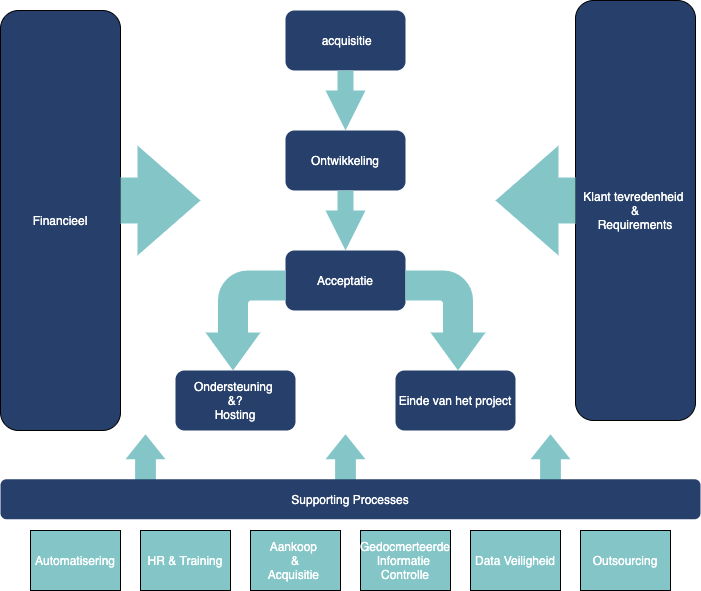
\includegraphics[width=12cm]{gfx/ProcessFlow}
\caption{Project Process}
\label{fig:Project Process}
\end{figure}

Naast het ontwikkelproces zijn er een aantal supporting processen die ervoor zorg dragen dat het bedrijf blijft draaien. Onder deze processen valt ook automatisering die voor ondersteuning zorgt van platformen waarop ontwikkeld en/of gehost wordt. Eaglescience ontwikkeld en genereert inkomsten op projectbasis. Alle processen die draaien moeten dus direct ingezet kunnen worden op projecten van klanten (figuur~\ref{fig:Project Process}). Als er een project voor intern gebruik wordt ondernomen moet er een duidelijk beeld zijn of er op termijn winst mee te behalen valt.

\section{Relevante en actuele ontwikkelingen binnen Eaglescience}\label{sec:relevante-en-actuele-ontwikkelingen-binnen-Eaglescience}

Eaglescience is aan het groeien, zowel in het aantal projecten als in het aantal medewerkers. Daarnaast worden de diensten die Eaglescience aanbied ook uitgebreid, en wordt het hosten van de ontwikkelde applicaties steeds vaker aangeboden. Door deze inzet ligt de verantwoordelijkheid niet alleen bij het leveren van een veilige en hoogwaardige software, maar ook bij het leveren van een veilige hosting service. Naast de groei van het bedrijf is ook de uitbreiding van diensten die aangeboden worden een reden om taken die geautomatiseerd kunnen worden dan ook te automatiseren.

Daarnaast heeft Eaglescience de afgelopen jaren een portfolio van verschillende klantproducten opgebouwd. Deze producten worden gehost, onderhouden en er wordt service en support geboden richting gebruikers. Eaglescience is momenteel dit onder de noemer Software Lifecycle Management aan het integreren in het kwaliteitssysteem door middel van beleid en het vastleggen in werkprocessen. Het in de grip en up-to-date houden van de live softwareproducten vraagt om een gerichte-, transparante- en traceerbare aanpak ten aanzien van alle gebruikte software-onderdelen (bibliotheken/ libraries) en onderliggende afhankelijkheden (dependencies).



 % Chapter 1
% Chapter 2

\chapter{Opdracht}\label{ch:opdracht} % Chapter title
Tegenwoordig zijn software-bibliotheken niet meer weg te denken uit het huidige software-ontwikkelproces. Bibliotheken geven ontwikkelaars de mogelijkheid code te hergebruiken in meerdere projecten, om zo efficiënter te kunnen ontwikkelen. Dit helpt op zijn beurt om de time-to-market te verkorten. Bibliotheken kunnen door bedrijven zelf geschreven worden, in het geval van Eaglescience is dit ArchES, of worden overgenomen van andere bedrijven/instellingen. ArchES is echter zelf ook afhankelijk van een aantal bibliotheken die niet ontwikkeld zijn door Eaglescience. Hierdoor kan niet worden voorkomen dat bibliotheken worden gebruikt waarvan de afkomst niet geheel kan worden herleid.

Deze (deels) onherleidbare bibliotheken vallen onder de noemer "Software of Unknown Provenance / Pedigree (SOUP)". Door het gebruik van dit soort bibliotheken kan er een aannemelijk risico ontstaan op het gebied van kwetsbaarheden. Om inzicht te verkrijgen in deze kwetsbaarheden en daarmee mogelijke veiligheidsissues dient een SOUP-analyse gedaan te worden. Binnen Eaglescience wordt het belang hiervan onderstreept en daarom wordt er gezocht naar een efficiënte en, waar mogelijk, geautomatiseerde manier voor het uitvoeren van een dergelijke analyse. Hierdoor kan de veiligheid van de ontwikkelde applicaties worden gewaarborgd zonder afbreuk te doen aan kwaliteit.

\section{Opdracht vanuit Eaglescience}\label{sec:opdracht-vanuit-Eaglescience}

Vanuit de CTO is de wens ontstaan om een systematisch opgebouwde methode te ontwikkelen waarbij er automatisch periodiek een SOUP-analyse gedaan wordt op bestaande en nieuwe projecten. Het beoogde resultaat is een module die wordt toegevoegd aan de al bestaande portal van Eaglescience waarbij project verantwoordelijken inzicht kunnen verkrijgen in de kwetsbaarheden die in een project aanwezig kunnen zijn door het gebruik van externe bibliotheken.

De aanleiding van deze opdracht is een gebrek aan inzicht in reeds draaiende software. In tegenstelling tot software waaraan nog ontwikkeld wordt, gaat er bij projecten waaraan niet actief wordt ontwikkeld het inzicht in gebruikte bibliotheken en hun versies verloren. Hierdoor is het onbekend welke kwetsbaarheden er mogelijk zijn in deze projecten.
\subsection{Eisen aan de opdracht}\label{subsec: eisen-aan-de-opdracht}
Vanuit Eaglescience worden er een aantal eisen gesteld waaraan het eindproduct moet voldoen. Als er aan deze eisen is voldaan is er voor Eaglescience een waardevol product ontwikkeld welke in gebruik kan worden genomen. Daarnaast zijn er een aantal opleveringseisen die gehaald dienen te worden om de kwaliteit te waarborgen. Ook is er aangegeven dat er bij voorkeur naar open source tooling dient gekeken te worden, daar er geen budget voor aanschaf van software voor handen is.
\newpage

\textbf{Functionele eisen}
\begin{itemize}
\item De module dient eenvoudig te kunnen worden gebruikt in de huidige Continuous Integration /Continuous Deployment (CI/CD) pipeline voor bestaande en nieuwe projecten
\item De module dient gebruik te maken van de bestaande huidige projectstructuur van de portal
\item De module dient ondersteuning te bieden aan meerdere omgevingen (OTAP)
\item De module dient te worden ontwikkeld in Angular en Play (Scala), zodat het in de bestaande portal module past
\item De module dient met een instelbaar interval de analyse uit te voeren
\item De module moet op project en omgeving niveau rapporteren over bekende kwetsbaarheden
\item De module dient kwetsbaarheden op minimaal drie niveau’s in te schalen (kritisch, gemiddeld en laag)
%\item De module dient ondersteuning te bieden voor het instellen van quality gates ten aanzien van de melding die het vind van ieder niveau, per project, per omgeving
\end{itemize}
\textbf{Kwaliteitseisen}
\begin{itemize}
\item De module dient te voldoen aan de geldende kwaliteitsnormen binnen Eaglescience, minimaal meetbaar door:
	\begin{itemize}
	\item Test coverage > 70\%
	\item Onderdeel van de bestaande CI/CD voor de Eaglescience Portal
	\end{itemize}
\item De geschreven code dient gereviewd te worden door een Eaglescience ontwikkelaar
\item De module dient gescheiden componenten te bevatten: Frontend, Backend, API
\item Voor de API dient gebruik te worden gemaakt van swagger
\item De module dient goed gedocumenteerd te zijn middels 'in code comments'
\end{itemize}

\subsection{Deliverables vereiste resultaten}\label{subsec:deliverables-vereiste-resultaten}
Vanuit de CTO worden er naast de functionele eisen ook eisen gesteld aan de oplevering:
\begin{itemize}
\item Geïntegreerde en aantoonbaar werkende module
\item De code van de module is gepubliceerd in Eaglescience GitLab
\item Aanwezigheid van een handleiding over hoe de module gebruikt dient te worden
\item Eventuele aanvullende deliverables vanuit de HvA
\end{itemize}

\section{Gewenst neveneffect}\label{sec:gewenst-neveneffect}
Naast dat de nieuwe module inzicht moet geven in de kwetsbaarheden van bibliotheken van derden zal deze ook bewustzijn creëren in risico's van het gebruik hiervan. Voordat er zal worden overgegaan tot het gebruik van een bibliotheek dienen de volgende vragen te worden beantwoord:
\begin{itemize}
	\item Is deze bibliotheek echt nodig?
	\item Zo ja, welke invloed heeft dat op de veiligheid van de applicatie?
	\item Kan deze functionaliteit ook op een andere eenvoudige manier worden bewerkstelligd?
	\item Is er een andere bibliotheek die dezelfde functionaliteiten biedt?

\end{itemize}


\section{Opdracht fasen}\label{sec:opdracht-fasen}
Om de hierboven beschreven opdracht zo goed als mogelijk uit te voeren dient er eerst een onderzoek gedaan te worden naar begrippen binnen het domein SOUP, de ontwikkelomgeving van Eaglescience en daarnaast naar mogelijkheden om bibliotheken te screenen en te testen op kwetsbaarheden. Na de onderzoeksfase moet er een module ontwikkeld worden die deze mogelijkheid implementeert met inachtneming van de hierboven genoemde eisen.

\subsection{Fase 1: Onderzoek} \label{subsec:fase-1:-onderzoek}
Als eerste dient er onderzoek gedaan te worden naar de huidige situatie binnen Eaglescience waarbij er gekeken wordt naar de huidige dev-stack, de tooling, de werkwijze, als ook de huidige manier van uitrollen van applicaties. Daarna dient er een begrippen / literatuur onderzoek gedaan te worden binnen het domein SOUP om een goede kennis te vergaren over het domein om een basis te kunnen leggen voor een te implementeren module. Daarnaast dient er onderzoek gedaan te worden om te zien of er bibliotheken en resources zijn waar informatie over SOUP-bibliotheken te vinden is, en aan welke eisen deze bibliotheken moeten voldoen om kwetsbaar te worden. Hier lettende op de eisen vanuit Eaglescience en de mogelijkheden die deze analyse bibliotheken bieden. Deze fase wordt beschreven in het deel~\ref{prt:Onderzoek} van dit document.

\subsection{Fase 2: Oplevering SOUP analyse module}\label{subsec:fase-2:-oplevering-soup-analyse-module}
De uit het onderzoek behaalde resultaten aangaande beschikbare resources om een SOUP-analyse uit te voeren vormen een leidraad voor de implementatie van de module. Deze module moet voldoen aan de eisen die gesteld zijn. Het ontwerp wordt beschreven in deel~\ref{prt:ontwerp}

\cleardoublepage % Empty page before the start of the next part

%------------------------------------------------

\part{Onderzoek}\label{prt:Onderzoek} % Second part of the thesis
\chapter{Onderzoeksplan}\label{ch:onderzoekPlan}

In het vorige hoofdstuk is de opdracht voor dit onderzoek beschreven. In dit hoofdstuk wordt uitgewijd over hoe deze opdracht en het daarbij behorende onderzoek zal worden uitgevoerd en welke bronnen er hiervoor gebruikt worden. Het resultaat is een onderzoeksplan voor een onderzoek naar analyses op kwetsbaarheden in externe bibliotheken (SOUP) binnen Eaglescience.


\section{Aanleiding}\label{sec:OP_aanleiding}
Eaglescience heeft de ambitie om te groeien in zowel het aantal projecten dat het aanneemt als in het aantal medewerkers. Daarnaast is het bezig met het integreren van het software lifecycle management paradigma in het kwaliteitssysteem om zo een gerichte-, transparante en traceerbare aanpak te hebben aangaande de kwaliteit en daarmee de veiligheid van de te leveren software. Er wordt gezocht naar manieren om taken die veel voorkomen en bijdragen aan de kwaliteit te automatiseren om op die manier een traceerbare en transparante aanpak te verkrijgen. Op dit moment mist voornamelijk inzicht in de kwetsbaarheden van projecten waarvan de ontwikkeling is afgerond, maar die wel door Eaglescience worden gehost en daardoor onder haar verantwoordelijkheid vallen.


\section{Probleemanalyse}\label{sec:probleemanalyse}
Eaglescience doet veel om veilige applicaties te leveren aan haar klanten. Tijdens het ontwikkelproces wordt er door de ontwikkelaars continue afgewogen welke maatregelen, in architectuur en/of code, moeten worden genomen om applicaties veilig op te kunnen leveren. Deze afwegingen zijn onderdeel van het ontwerpproces en worden door de klant gezien als declarabele uren en zij zijn dan ook bereid voor deze werkzaamheden te betalen. Op het moment dat een project 'klaar' is en over gaat van ontwikkeling naar hosting wordt er onderhoud gedaan volgens afspraken in de SLA. In diezelfde SLA wordt niet altijd ruimte opgenomen voor het testen van de applicatie op kwetsbaarheden middels SOUP-analyses. Vaak komt dit doordat de klant er geen budget voor heeft, of het niet belangrijk vindt. Gezien Eaglescience alleen een advies kan uitbrengen over support en de klant de eindbeslissing neemt worden SOUP-analyses vaak niet of niet tijdig uitgevoerd. Omdat Eaglescience wel "zo veel mogelijk" wil garanderen dat de software die gehost wordt veilig is, dient de applicatie in hosting periodiek geanalyseerd te worden op kwetsbaarheden. Op dit moment is dit een tijdrovend handmatig process waarmee een teamlid ongeveer 8 tot 12 uur bezig is. Voor iedere dependency moet er namelijk bekeken worden of er mogelijke kwetsbaarheden bestaan, of dan al niet geupdate moeten worden. Door de groei die Eaglescience binnenkort wil maken bestaat de wens om bovenstaand proces te automatiseren.

Er moet dus een methode worden ontwikkeld die het mogelijk maakt om geautomatiseerd en periodiek een SOUP-analyse te doen op dependencies binnen een project. De SOUP-analyses moeten inzichtelijk maken of en zo ja, welke, kwetsbaarheden zijn gevonden in deze bibliotheken. De methode moet voor alle platformen (Docker, programmeertalen, databases etc.) dezelfde resultaten geven, en compatibel zijn met de huidige infrastructuur van Eaglescience.

Door de analyses te automatiseren wordt beoogd dat er minder tijd zal hoeven te worden besteed aan de analyse. Deze tijd kan dan worden ingezet door de ontwikkelaar aan taken die declarabel zijn en voor beide partijen winstgevend zijn.


\section{Probleem stelling, onderzoeksvraag en doelstellingen}\label{sec:probleem-stelling-onderzoeksvraag-en-doelstellingen}
Samengevat luidt het probleem: Het handmatig uitvoeren van SOUP-analyses kost manuren die niet declarabel zijn. Om deze reden is de wens dat er een geautomatiseerde oplossing komt die periodiek de projecten, die in ontwikkeling zijn en/of door Eaglescience gehost worden, analyseert op kwetsbaarheden in gebruikte externe bibliotheken. Door deze automatische oplossing te gebruiken wordt beoogd dat de (niet declarabele) uren die normaal gebruikt worden voor het analyseren van projecten in plaats daarvan gebruikt kunnen worden voor andere wel declarabele uren. Hierdoor zou de efficiëntie binnen Eaglescience kunnen worden verhoogd.

Voor het onderzoek naar het hierboven genoemde probleem is de volgende centrale onderzoeksvraag opgesteld: "Hoe kan Eaglescience middels een geautomatiseerde methode inzicht krijgen in potentiële kwetsbaarheden van gebruikte bibliotheken binnen projecten, waarbij rekening gehouden wordt met de huidige manier van werken?"

De opdracht heeft de volgende doelstelling:
Het doel van dit onderzoek is het ontwikkelen van een methode om SOUP-analyses uit te voeren binnen de dev-stack van Eaglescience. Hierbij moet rekening gehouden worden met de in de opdracht gegeven criteria. Aan het einde van het onderzoek moet een methode worden gepresenteerd die vervolgens bewezen kan worden middels een implementatie van een analyse op de twee meest gebruikte technologieën binnen Eaglescience, Scala en TypeScript.


\section{Stakeholderanalyse}\label{sec:stakeholdersanalyse}
Om inzicht te verkrijgen in het draagvlak voor dit onderzoek dient er een stakeholders analyse gedaan te worden. Op deze manier moet het duidelijk worden wie de stakeholders zijn en welke belangen zij hebben bij het doen van een onderzoek naar een geautomatiseerde SOUP-analyse en de resultaten hiervan.

\subsection{Dagelijks bestuur (intern)}\label{subsec:dagelijks-bestuur-(intern)1}
Het dagelijks bestuur ziet vooral voordelen in het op een overzichtelijke manier verkrijgen van inzichten in kwetsbaarheden. Zij beogen dat ze hierdoor beter kunnen aansturen in het gebruik van bibliotheken en/of andere technologieën. Ondanks dat de ontwikkeling van de beoogde nieuwe module vooral geld zal kosten, is de huidige manier van werken ook niet kosten-effectief. Daarnaast voorziet de CTO dat de nieuwe module tijdswinst zal opleveren waardoor de time-to-market voor andere projecten hoger kan komen te liggen en er dus op langere termijn meer omzet gegenereerd kan worden.

\subsection{Projectmanagers (intern)}\label{subsec:projectmanagers-(intern)1}
Projectmanagers krijgen op dit moment een update over de staat van kwetsbaarheden na afronding van een analyse, welke vaak na een deploy plaatsvindt of op verzoek. De nieuwe module zal echter de mogelijkheid bieden om up-to-date informatie on-demand te verkrijgen.
De tijdsinvestering die nodig is van ontwikkelaars voor de ontwikkeling van de module weegt volgens hen op tegen de voordelen die de module in de toekomst kan brengen.

\subsection{Ontwikkelteam (intern)}\label{subsec:ontwikkelteam-(intern)1}
Het handmatig testen van kwetsbaarheden werd tot op vandaag gedaan door het ontwikkelteam. Dit is een tijdrovende taak, welke ten koste gaat van de ontwikkeling van software voor klanten. Het ontwikkelteam heeft daarom direct baat bij de ontwikkeling van de beoogde module en wil daarom graag hieraan meedenken en meewerken.

\subsection{Klant (extern)}\label{subsec:klant-(extern)1}
De enige externe stakeholder is de klant, welke ook een passieve stakeholder is, gezien zij niet direct betrokken zijn bij de ontwikkeling van de module, maar wel baat hebben bij de uitkomst hiervan, namelijk in de vorm van veiligere en betrouwbaardere software tegen potentieel lagere kosten.

\begin{figure}
    \myfloatalign
    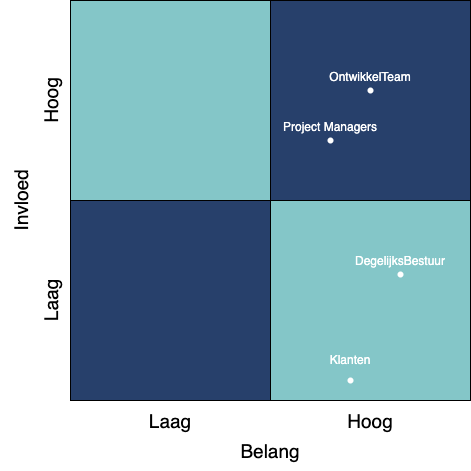
\includegraphics[width=10cm]{gfx/stakeholderanalyse}
    \caption{StakeHolders Analyse}
    \label{fig:StakeholderAnalyse1}
\end{figure}
Zoals te zien is in figuur~\ref{fig:StakeholderAnalyse1} is hebben alle stakeholders veel baat bij een nieuwe module voor de analyse van kwetsbaarheden. De invloed hierop is het hoogst bij het ontwikkelteam en de projectmanagers. De lage invloed van de klant zorgt ervoor dat voor het ontwerp alleen de requirements vanuit Eaglescience worden opgenomen.

\section{Theoretisch kader}\label{sec:theoretisch-kader}
Het theoretisch kader waarmee wordt gewerkt bestaat uit twee delen. Het eerste deel omvat theorie over externe bibliotheken. Het richt zich op het gebruik hiervan en de potentiële gevaren en methoden om deze bibliotheken te analyseren. De geselecteerde bronnen zijn:
\begin{itemize}
    \item \textbf{OWASP top 10}
    De OWASP Top-10 is als uitgangspunt gekozen omdat de inhoud van dit document binnen Eaglescience geldt als aandachtspunt voor het ontwikkelen van veilige software. De basis voor dit onderzoek wordt beschreven in punt "A06:2021-Vulnerable and Outdated Components". Hier wordt beschreven welke gevaren er potentieel dreigen als op dit punt niets gedaan wordt~\citep{OWASP:2021}.
    \item \textbf{OWASP dependency-check} Pagina over het project binnen de OWASP voor het analyseren van componenten in applicaties~\citep{OWASP:2017}.
    \item \textbf{Justifying the use of software of uncertain pedigree (SOUP) in safety-related applications} Hoewel dit document verouderd lijkt staat er wel degelijk interessante informatie over waarom je SOUP zou gebruiken en hoe je de risico's kan verminderen~\citep{Bischop:2001} .
    \item \textbf{Backstabber’s Knife Collection: A Review of Open Source Software Supply Chain Attacks}Dit artikel bevat informatie over een mogelijke vorm van aanvallen die middels SOUP uitgevoerd zouden kunnen worden. Daarnaast geeft het artikel inzicht in hoe de onderzoekers packages voor NPM, Python, en Ruby hebben onderzocht op kwetsbaarheden~\citep{Ohm:2020}.
\end{itemize}
Het tweede deel omvat de werkwijze van Eaglescience en de door hun gebruikte technologieën. De geselecteerde documenten vormen de basis informatie over de werkwijze van Eaglescience en zal als input worden gebruikt bij het ontwerp van de analyse die aansluitend aan het onderzoek zal plaatsvinden. De volgende bronnen zullen bij het onderzoek worden gebruikt:
\begin{itemize}
    \item \textbf{151030 F04B Proces Flow Chart ES\_V1.0\_TN.pdf} Een document dat de workflow beschrijft die binnen Eaglescience gehanteerd wordt~\citep{Eaglescience:2015}.
    \item \textbf{200121\_Policy Manual\_ES\_V6 signed.pdf} ISO-handboek waarin de bedrijfsvoering binnen Eaglescience wordt beschreven~\citep{Eaglescience:2020}.
\end{itemize}

\section{Conceptueel model}\label{sec:conceptueel-model}
Om de relevantie en relatie van de verschillende onderzoeken te waarborgen is een conceptueel model opgesteld(figuur~\ref{fig:ConceptueelModel}).
\begin{figure}
    \centering
    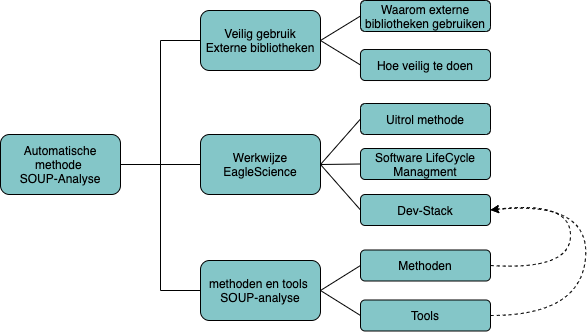
\includegraphics[width=12cm]{gfx/Conceptueel Model}
    \caption{Conceptueel Model}
    \label{fig:ConceptueelModel}
\end{figure}
Dit model maakt de samenhang van de verschillende begrippen inzichtelijk. Het kernbegrip is "Automatische methode SOUP-analyse" welke dit onderzoek uiteindelijk moet opleveren. Om hiertoe te komen zijn er drie begrippen die ieders een eigen domein binnen de probleemstelling belichten. In het theoretisch deel "Veilig gebruik externe bibliotheken"  wordt onderzocht waarom er bibliotheken van buitenaf worden gebruikt en wat de potentiële gevaren zijn die dit met zich meebrengt, en eventuele remedies hiervoor. Daarna zal "Werkwijze Eaglescience"  de manier van werken binnen Eaglescience belichten als ook de manier van uitrollen en de algehele dev-stack die Eaglescience gebruikt. Het begrip "Methoden en tools SOUP-analyse" zal ingaan op de beschikbare tools die gebruikt kunnen worden om een analyse te doen. Met deze tools wordt een methode onderzocht die SOUP-analyses mogelijk maakt binnen de dev-stack van Eaglescience. Samen zal dit onderzoek leiden tot een theoretische methode die als input kan gelden voor het ontwerp voor de nieuwe module die in de opdracht staat beschreven.

\section{Onderzoeksontwerp}\label{sec:OP_onderzoeksontwerp}
Aan de hand van de hierboven beschreven doelstellingen, theoretisch kader en conceptueel model is het volgende onderzoeksontwerp opgesteld.

\subsection{Onderzoeksvraag}\label{subsec:onderzoeksvraag-en-deelvragen}
Op basis van de probleemanalyse luidt de onderzoeksvraag als volgt: "Hoe kan Eaglescience middels een geautomatiseerde methode inzicht krijgen in potentiële kwetsbaarheden van gebruikte bibliotheken binnen projecten waarbij rekening gehouden wordt met de huidige manier van werken?". Door het ontleden van deze onderzoeksvraag ontstaan er twee delen waarnaar onderzoek gedaan moet worden. Het eerste deel is het gebruik en gevaar van externe bibliotheken, welke leidt tot de volgende onderzoeksvraag: "Wat is het effect van het gebruik van externe bibliotheken bij het ontwikkelen van software, welke gevaren brengt dit met zich mee en wat kan er gedaan worden om deze gevaren te minimaliseren?". Vervolgens kan deze kennis worden benut in het tweede deel, wat de praktische kant belicht, gericht op de methode en tooling voor SOUP-analyses. Dit tweede deel omvat methodes om geautomatiseerd SOUP-analyses te doen op projecten binnen Eaglescience. De onderzoeksvraag luidt als volgt: "Welke SCA tooling is compatibel met de omgeving van Eaglescience en welke methode kan worden toegepast om deze tooling te gebruiken voor het automatisch analyseren van externe dependencies?"

Deze delen zullen ieders in een deelonderzoek worden behandeld, waarvan de uitkomsten elkaar zullen aanvullen en samen tot een eind eindresultaat leiden.
\begin{figure}
    \myfloatalign
    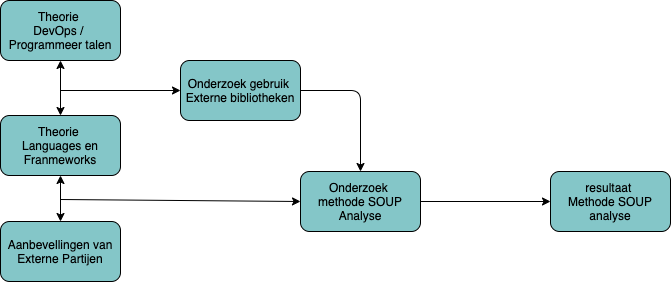
\includegraphics[width=12cm]{gfx/Onderzoekmodel}
    \caption{Onderzoeksmodel}
    \label{fig:OnderzoeksModel}
\end{figure}

In figuur\ref{fig:OnderzoeksModel} is te zien hoe de twee onderzoeken met elkaar in relatie staan ten opzichte van het beoogde eindresultaat. Het onderzoek over het gebruik van externe bibliotheken zal leiden tot concrete inzichten die vervolgens gebruikt kunnen worden als kennis in het onderzoek naar een methode voor een SOUP-analyse. Dit zal uiteindelijk een methode opleveren die gebruikt kan worden voor de implementatie van de module die aan de opdracht voldoet.

\subsection{Scope}\label{subsec:scope}
Het domein softwareveiligheid is op het moment van schrijven een 'hot-topic', en zeer breed. Om deze reden is er gekozen om dit onderzoek te beperken tot het veiliger maken van software middels het analyseren en beschikbaar stellen van informatie over externe bibliotheken. Daarnaast zullen alleen de technologieën die compatibel zijn met de werkwijze van Eaglescience mee worden genomen. Daarnaast is de opdracht zoals deze is gegeven door de CTO van Eaglescience de leidraad voor de scope van het onderzoek.

\subsection{Onderzoek strategie}\label{subsec:onderzoek-strategie}
Zoals hierboven is aangegeven zullen er een tweetal onderzoeken worden uitgevoerd. De conclusie van het eerste onderzoek zal dienen als input voor het tweede onderzoek.

%\newpage %TODO: quickfix om volgorde lijkheid te veranderen voor figuren...


\subsubsection{Onderzoek 1: gebruik externe bibliotheken, het gevaar en hoe veiliger te maken}
Het \textbf{doel} van dit onderzoek is om inzicht te krijgen in wat een SOUP-analyse is en hoe relevant het is om deze uit te voeren. Daarnaast wordt er gekeken wat de SOUP-analyse toevoegt aan de veiligheid van de software die Eaglescience levert en hoe Eaglescience mogelijk kan voorkomen dat er kwetsbaarheden in de uitgerolde software terecht komen.
De \textbf{scope} van dit onderzoek is dat er gekeken wordt naar het gebruik van externe bibliotheken en de toegevoegde waarde hiervan. Daarnaast wordt er gekeken wat er gedaan kan worden om het gebruik van externe bibliotheken veiliger te maken.
De \textbf{onderzoeksvraag} luid: "Wat is het effect van het gebruik van externe bibliotheken bij het ontwikkelen van software, welke gevaren brengt dit met zich mee en wat kan er gedaan worden om deze gevaren te minimaliseren?".
De gebruikte \textbf{methodes} zullen deskresearch zijn aangevuld met conferenties, waarbij \textbf{bronnen} zoals artikelen en rapportages van instanties en bedrijven die zich bezighouden met de veiligheid van software zullen worden opgenomen met als focus het gebruik van externe bibliotheken. Software veiligheid is een 'hot-topic' en er worden jaarlijks veel conferenties gehouden over dit onderwerp. Door de huidige wereld situatie is het mogelijk om veel van deze conferenties  ''on-demand'' terug te kijken wat op zijn beurt ook weer tot andere inzichten kan leiden. In figuur~\ref{fig:OnderzoeksModelNoodZaakSOUP} is te zien hoe het onderzoek is opgebouwd.
\begin{figure}[htbp]
    \myfloatalign
    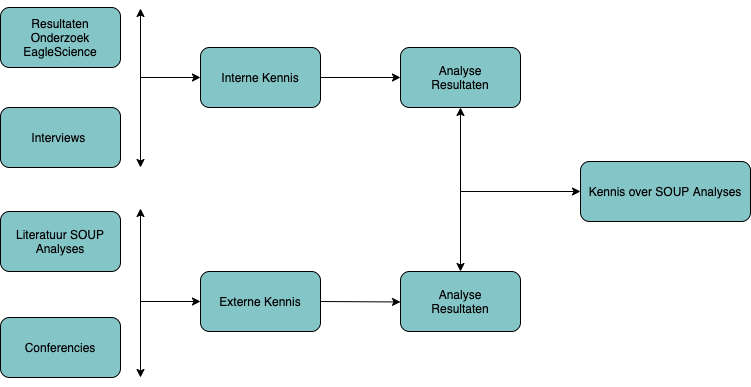
\includegraphics[width=12cm]{gfx/OnderzoeksmodelSOUP}
    \caption{Onderzoeksmodel gevaren van SOUP}
    \label{fig:OnderzoeksModelNoodZaakSOUP}
\end{figure}



\subsubsection{Onderzoek 2: tools en methodes voor SOUP-analyses op de Eaglescience dev-stack}
Het \textbf{doel} van dit onderzoek is om een methode te vinden die het mogelijk maakt om een SOUP-analyse te doen binnen de huidige dev-stack van Eaglescience. Hiervoor zullen er geschikte SCA (Software Composition Analysis) tools gevonden moeten worden. Binnen de \textbf{scope} van het onderzoek zal daarom alleen gekeken worden naar SCA tooling die analyses doet voor componenten binnen de dev-stack van Eaglescience. De \textbf{onderzoeksvraag} luidt: "Welke SCA tooling is compatibel met de omgeving van Eaglescience en welke methode kan worden toegepast om deze tooling te gebruiken voor het automatisch analyseren van externe dependencies?". De \textbf{methode} die gebruikt wordt is deskresearch. Daarnaast zullen er interviews gehouden worden met collega's om inzicht te krijgen in de huidige stand van zaken op het gebied van gebruik van externe bibliotheken en hoe er in de huidige situatie voor wordt gezorgd dat er geen kwetsbaarheden worden geïntroduceerd door het gebruik hiervan. Als er een selectie is gemaakt voor een tool dient deze in een kleine testopstelling getest te worden om vervolgens te kijken of deze kan worden geïmplementeerd in de bestaande uitrol methode. De \textbf{bronnen} die gebruikt zullen worden zijn informatie bronnen van leveranciers van dergelijke tooling. Ook zal er in interne documentatie worden gekeken hoe de huidige processen draaien waarin wordt beoogd om de SOUP-analyse uit te voeren. Daarnaast zullen de bevindingen middels een review worden geverifieerd op bruikbaarheid bij de opdrachtgever. Het onderzoeksmodel voor dit onderzoek is te vinden in figuur~\ref{fig:OnderzoeksModelSOUPmethode}.

\begin{figure}[htbp]
    \myfloatalign
    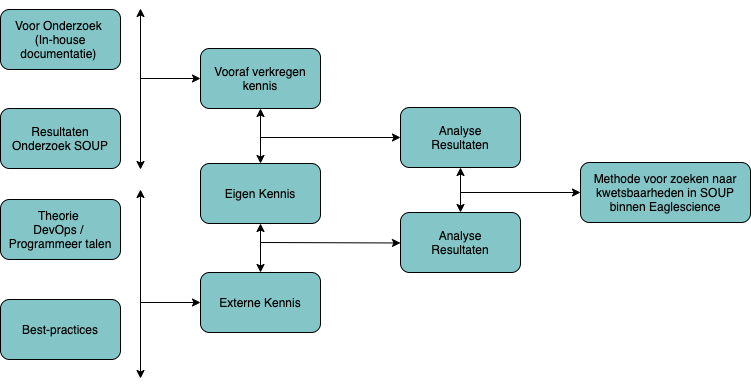
\includegraphics[width=12cm]{gfx/OnderzoeksModelSOUPMethode}
    \caption{Onderzoeksmodel SOUP-analyse module}
    \label{fig:OnderzoeksModelSOUPmethode}
\end{figure}

\section{Planning}\label{sec:planning}
Om tijdig tot resultaten te komen is de volgende planning opgesteld.

\subsection{Requirements analyse \textbf{september 2021}}\label{subsec:requirements-analyse}
Na het ontvangen van de opdracht dient er onderzocht te worden of er naast de eisen die door de CTO in de opdracht zijn gezet nog andere eisen zijn binnen Eaglescience. Hiervoor zal er onderzocht worden welke betrokkenen er zijn en welke belangen en wensen zij hebben. Na het houden van interviews zullen alle wensen tegen elkaar worden afgewogen. Dit zal leiden tot een document waarin alle belangrijke requirements worden geprioriteerd volgens de MoSCoW\-methode.

\textbf{Methode:} Intake gesprek met opdrachtgever, interviews met betrokkenen, enquete voor ontwikkelaars.

\textbf{Resultaat:} Applicatie requirements document.

\subsection{Vooronderzoek \textbf{september 2021 - oktober 2021 }}\label{subsec:onderzoek}
Om de requirements om te kunnen zetten naar een ontwerp zal er onderzoek gedaan worden naar de huidige manier van ontwikkelen en compileren van de software. Een onderzoek naar begrippen binnen het domein SOUP is een voorwaarde om vervolgens onderzoek te kunnen doen naar methodes om analyses te kunnen doen op software die Eaglescience maakt ten opzichte van SOUP. De resultaten van het vooronderzoek zullen worden gebruikt als input.
Om meer kennis en verdieping te krijgen in de materie rondom de nieuwe module zullen er een aantal onderzoeken worden uitgevoerd.


Er is onderzoek nodig naar de volgende onderwerpen:
\begin{itemize}
    \item \textbf{Externe bibliotheken gebruik en het gevaar}: Onderzoek naar waarom er externe bibliotheken worden gebruikt en het gevaar hiervan en hoe deze kunnen worden ondervangen.
    \item \textbf{SOUP Analyse binnen Eaglescience}: Dit onderzoek zal de tooling en methode in kaart brengen voor het uitvoeren van SOUP\-analyses binnen Eaglescience.
\end{itemize}

\textbf{Methode:} Bureau onderzoek, interviews met specialisten, deelnemen aan en/of terugkijken van conferenties, Sandbox testen met gevonden tooling.

\textbf{Resultaat:} Inzicht in het begrip SOUP en software veiligheid als ook een idee voor een mogelijke implementatie van de oplossing die voor Eaglescience de beste is zonder veel impact op de huidige manier van werken te hebben.

\subsection{Initieel ontwerp \textbf{oktober 2021 - november 2021 }}\label{subsec:initieel-ontwerp}
Er zal een ontwerp worden gemaakt waarin vast gelegd is welke requirements er beslist in de module moeten zitten en de uitwerking van deze. Evenals een ontwerp van de architectuur en het datamodel. Naast de module zal er ook een ontwerp gemaakt worden voor een ontwikkel/test omgeving om de module continue te kunnen testen zonder dat dit de huidige buildstraat beïnvloed. Dit laatste is van belang om zo min mogelijk storingen te veroorzaken in de dagelijkse gang van zaken bij al lopende projecten. Het eerste ontwerp zal als leidraad dienen voor de implementatie waarin afgeweken kan worden als dit nodig blijkt tijdens de implementatie sprints.

\textbf{Methode:} Overleggen met ontwikkelaars, huidige omgeving onderzoeken op mogelijkheden en architectuur.
\textbf{Resultaat:} Eerste ontwerp in de vorm van een datamodel, blokdiagram van architectuur voor de oplossing, als ook een sequentiediagram om van analyse tot rapportage te komen.

\subsection{Implementatie en Testen \textbf{november 2021 - januari 2022 }}\label{subsec:implementatie-en-testen}
Om te kunnen beginnen aan de implementatie is er een ontwikkel/ test omgeving nodig die het mogelijk maakt om zonder invloed op de dagelijkse werkzaamheden van Eaglescience een module te kunnen ontwikkelen. Deze zal eerst worden opgezet. Als test projecten zullen snapshots worden gebruikt van de daadwerkelijke projecten dit om een zo accuraat mogelijke test omgeving te hebben. Zoals in de opdracht beschreven dient de nieuwe module een onderdeel te zijn van de bestaande portal. Er zal dan ook direct samen worden gewerkt met het team die daar op het moment mee aan het ontwikkelen is. Tijdens de implementatie zal er ook worden gedocumenteerd wordt hoe de module werkt en welke procedures hier in worden gevolgd. Dit document biedt ontwikkelaars de mogelijkheid om dit door te nemen als on-boarding en referentie.

\textbf{Methode:} Agile scrum sprints met iedere 2 weken een oplevermoment en demo als ook een reflectie op de sprint.
\textbf{Resultaat:} Werkende en geteste applicatie die klaar is om uitgerold te worden.

\subsection{Uitrollen en documentatie \textbf{januari 2022 - februari 2022 }}\label{subsec:uitrollen-en-documentatie}
Nadat de implementatie van de meest kritische requirements is afgerond zal er worden begonnen met het uitrollen van de module en het testen door een geselecteerde groep gebruikers. De feedback wordt bekeken en meegenomen in de evaluatie. Mocht het nodig zijn dan zal er acuut actie worden ondernomen om deze wijzigingen aan te passen. Mochten er wensen zijn die kunnen wachten dan zal er worden overwogen om deze mee te nemen in de volgende iteratie van het project. Daarnaast zal ook de documentatie verder worden afgerond.
\textbf{Methode:} Interviews met stakeholders met een analyse over de nieuwe requirements.

\textbf{Resultaat:} Uitgerolde en gedocumenteerde applicatie.


\chapter{Onderzoek: Het gevaar van het gebruik van externe bibliotheken}\label{ch:externeBibliothekengebruikGevaren}
Voordat er een methode voor het analyseren van externe bibliotheken op kwetsbaarheden kan worden ontwikkeld is theoretische kennis over het gebruik van externe bibliotheken, het gevaar hiervan en op welke manier er veilig mee gewerkt kan worden noodzakelijk. De onderzoeksvraag voor dit onderzoek luidt dan ook: $"$Wat is het effect van het gebruik van externe bibliotheken bij de ontwikkeling van software, welke gevaren brengt het gebruik hiervan met zich mee en wat kan er gedaan worden om deze gevaren te minimaliseren?$"$. Deze onderzoeksvraag is op te delen in de volgende deelvragen die ieders in een eigen sectie zullen worden behandeld.

\begin{itemize}
    \item Wat zijn externe componenten en waarom worden deze vaak SOUP genoemd?
    \item Waarom en hoe vaak worden externe bibliotheken gebruikt in het ontwikkelen van software?
    \item Wat zijn potentiële gevaren die bij het gebruik van externe bibliotheken kunnen worden geïntroduceerd?
    \item Hoe kunnen applicaties weerbaarder worden gemaakt tegen kwetsbaarheden die gepaard gaan met het gebruik van externe bibliotheken?
\end{itemize}
De uitkomsten hiervan zullen als input worden gebruikt voor het onderzoek naar een methode voor SOUP-analyses binnen Eaglescience. Daarnaast zullen de in dit onderzoek verkregen inzichten worden gedeeld met collega's om bewustwording over dit onderwerp te vergroten. De methode die voornamelijk gebruikt zal worden voor dit onderzoek is deskresearch. Dit zal worden aangevuld met het volgen van webinars.

\section{Wat zijn externe componenten en waarom worden deze ook wel SOUP genoemd?}\label{sec:watisSOUP}
Kort door de bocht zijn externe componenten, componenten die niet door het bedrijf zelf zijn ontwikkeld. Enkele voorbeelden hiervan zijn operating systems, runtime omgevingen, Docker images, database management systemen, bibliotheken en frameworks. Vaak zijn deze componenten open-source, al dan niet ontwikkeld door een community.
Op het moment dat er van een component niet kan worden achterhaald op welke manier en door wie deze ontwikkeld is wordt het $"$Software of Unknown Provenance (SOUP)$"$ genoemd. Dit begrip is ontstaan voor veiligheids intensieve applicaties, zoals software die gebruikt wordt in bv. ziekenhuizen, verkeersleiding, energieleveranciers etc.
Omdat de manier waarop deze componenten zijn ontwikkeld niet altijd duidelijk is kan er daardoor ook niet worden nagegaan of deze componenten aan de veiligheidseisen voldoen die de gebruiker stelt. SOUP kan worden herkend aan één of meerdere van de volgende kenmerken~\citep{Bischop:2001}:
\begin{itemize}
    \item Het moet al bestaan
    \item Het kan niet opnieuw worden ontwikkeld door de gebruiker
    \item Het is generiek en bevat mogelijk functies die niet toepasbaar zijn in de te ontwikkelen applicatie
    \item Het wordt geregeld aangepast om aan klantwensen en competitie te voldoen
\end{itemize}

Zeker in het geval van open-source is de manier van ontwikkelen niet altijd volledig gedocumenteerd en kan een groot deel van deze software onder de noemer SOUP worden geplaatst. Het gebruik van SOUP hoeft niet per definitie gevaarlijk te zijn, echter moet er wel worden opgelet hoe het gebruikt wordt, zoals hieronder verder zal worden besproken. In verband met de eerder besproken scope van het onderzoek zal er hierna enkel worden ingegaan op externe bibliotheken en frameworks.

\section{Waarom en hoe vaak worden externe bibliotheken gebruikt in ontwikkeling?}\label{sec:waarom-hoe}
Softwareontwikkeling staat altijd onder druk van deadlines en collega's of klanten die wachten op een feature. Daarom zijn er een aantal principes ontstaan die in de programmeerwereld als mantra worden aangenomen. Het eerste principe is KISS (Keep it simple, Stupid!): Probeer de componenten die je ontwikkeld zo simpel mogelijk te houden ondanks de complexiteit van de software. Het tweede principe is YAGNI (You ain't gonna need it) Ontwikkel de huidige requirements en probeer niet in de toekomst te kijken en hier al features voor te schrijven. Het derde en bovendien belangrijkste principe is DRY (Don't repeat yourself): Herhaling kost tijd die anders nuttiger kan worden besteed. Door functies op meerdere plekken te herhalen kunnen problemen worden ondervonden in de onderhoudbaarheid van de applicatie, omdat dezelfde methodes op meerdere plekken terug te vinden zijn. Datastructuren, functies, etc. die op verschillende plaatsen gedefinieerd zijn indicatoren tot een zekerheid van bugs. Dit omdat er de kans bestaat dat een ontwikkelaar vergeet een functie te updaten op een plek waar deze onverwacht ook gedefinieerd wordt~\citep{Papadopoulo:2021}.

Om deze mantra's te kunnen volgen bestaan er bibliotheken. Ze zorgen ervoor dat functies en datastructuren op één enkele plek worden gedefinieerd waardoor er ontwikkeltijd bespaard wordt wanneer een functie aangepast moet worden. Door gebruik van bibliotheken hoeft dit maar op een enkele plaats te gebeuren. Ook wordt er op deze manier gegarandeerd dat er maar een enkele versie bestaat van die functie of datastructuur.

In het geval van externe bibliotheken zijn er nog meer voordelen te benoemen. Bij het gebruik hiervan wordt de ontwikkeltijd uitbesteed of, in het geval van een bestaande bibliotheek, kan er zonder ontwikkeltijd functionaliteit worden overgenomen. Er is wel tijd nodig om deze functionaliteiten te implementeren, maar dat weegt niet op tegen de tijd die het kost om de functionaliteit zelf te ontwikkelen en te testen. Zeker in het geval van community driven bibliotheken wordt er veelvuldiger op functionaliteit getest, dan een individueel bedrijf kan doen op een zelf ontwikkelde bibliotheek.

Door boven genoemde voordelen worden externe bibliotheken vaak gebruikt. Volgens een onderzoek van Synopsys\footnote{Synopsys is een bedrijf dat zich bezig houdt met de ontwikkeling en verificatie van semiconductoren. Daarnaast ontwikkeld het tools voor verschillende taken in het domein software veiligheid.} bestond in 2020 ongeveer 98\% van de 1546 geanalyseerde codebases uit open-source componenten~\citep{Synopsys:2021}. Daarnaast bevatte 84\% van deze codebases minimaal één kwetsbaarheid met een gemiddelde van 158 kwetsbaarheden. De gemiddelde kwetsbaarheid was 2.2 jaar oud. Een ander belangrijk signalement dat Synopsys beschreef was dat er steeds meer codebases ontstonden welke tenminste één kwetsbaarheid bevatte.

Hiernaast heeft het bedrijf TideLift\footnote{TideLift is een bedrijf dat zich inzet voor het verbeteren van veilig gebruik van open-source software} meerdere onderzoeken gedaan naar hoe ontwikkelaars tegenover het gebruik van open-source componenten staan. Hun onderzoek wees uit dat ontwikkelaars over het algemeen eerder voor open-source kozen dan voor betaalde software. De redenen hiervoor waren onder andere: grotere flexibiliteit, snellere ontwikkeltijden, tevredenheid van de ontwikkelaar en een gunstiger kostenplaatje~\citep{TideLift:2021}. De enige reden die werd opgemerkt om voor betaalde software te kiezen was de beschikking over betere support en consultancy service. Op het gebied van software veiligheid gaf 61\% aan meer te vertrouwen op open-source software dan op aangekochte software.
Het onderzoek wees ook uit dat de selectie voor het gebruik van een open-source project vaak gedaan wordt op basis van hoe actief een project is, de betrouwbaarheid van de bron, en hoeveel mensen er aan het project werken.

Ook al zijn de cijfers hierboven beschreven afkomstig van afhankelijke bronnen, met een mogelijk conflict of interest, ze geven wel aan dat externe bibliotheken vaak worden gebruikt omdat dit vaak makkelijke, snel implementeerbare en mogelijk flexibele oplossingen biedt.

\section{Wat zijn potentiële gevaren bij het gebruik van externe bibliotheken?} \label{sec:wat-zijn-potentieel-gevaren-die-het-gebruik-van-externe-bibliotheken?}
Hoewel er enorme voordelen gepaard gaan met het gebruik van externe bibliotheken bij de ontwikkeling van software, zijn er ook een aantal nadelen te benoemen. De grootste is dat er potentieel kwetsbaarheden kunnen worden geïntroduceerd in de applicatie, welke niet of pas in een later stadium worden opgemerkt door ontwikkelaars die de bibliotheken gebruiken. Deze kwetsbaarheden kunnen zich op meerdere manieren manifesteren in de vorm van een $"$Supply Chain Attack$"$. Zoals de naam al doet vermoeden vindt er hierbij een aanval plaats middels functionaliteiten die zich in de dependencies bevinden. Deze aanval kan op verschillende manieren plaatsvinden, maar heeft meestal als doel een gewin voor de aanvaller. Hierbij kan er enerzijds op één of andere manier data bemachtigd worden, en anderzijds de functionaliteit van de doelapplicatie op een dusdanige manier worden aangetast dat deze in het voordeel is van de aanvallers. Een probleem met dit soort aanvallen is vaak dat deze lange tijd onopgemerkt kunnen blijven omdat externe bibliotheken niet periodiek worden gecheckt op juistheid, en worden gebruikt op basis van goed vertrouwen. Op het moment dat kwetsbaarheden al opgemerkt worden en hiervan een verslag wordt gemaakt in een vulnerability database (NIST, NVD, Mitre) duurt het nog geruime tijd voor deze door andere gebruikers worden opgemerkt en hierop actie wordt ondernomen. Hierdoor is de tijd waarin meerdere gebruikers bloot worden gesteld aan mogelijke kwetsbaarheden groot. Daarnaast gebruiken ook aanvallers de beschikbare informatie die de Vulnerability database bevat om verdere aanvallen mee te plannen.

Een ander nadeel van het gebruik van een externe bibliotheek is dat je niet zelf de verantwoordelijkheid hebt over de geschreven code en daarmee overgeleverd bent aan de ontwikkelaar daarvan voor het uitvoeren van updates om eventuele kwetsbaarheden te verwijderen. Wanneer dit niet gebeurd zal dit in eigen beheer moeten worden gedaan, of moet er worden gekozen voor een andere bibliotheek met vergelijkbare functionaliteiten.

Onderzoek van SonaType\footnote{SonaType is een bedrijf dat tools maakt voor software veiligheid} uitgevoerd in 2021 gaf aan dat er een jaar op jaar stijging was van 650\% in het aantal aanvallen gepleegd middels kwetsbaarheden in open-source bibliotheken~\citep{Sonatype:2021}.
Hiernaast bleek dat een groot deel van de applicaties niet wordt bijgewerkt, of vaak niet op de juiste manier, zodat er altijd een kwetsbaarheid zal blijven bestaan.

\section{Hoe kunnen applicaties weerbaarder worden gemaakt tegen kwetsbaarheden?}\label{sec:hoe-kan-er-voorkomen-worden-dat-er-kwetsbaarheden-ontstaan-in-een-applicatie-die-gebruik-maakt-van-externe-bibliotheken?}

Steeds meer bedrijven en instanties voelen zich verantwoordelijk voor de ontwikkeling van veiligere software, al dan niet vanuit een winstoogmerk. De OWASP is een stichting die zich voornamelijk bezig houdt met het verbeteren van software veiligheid met in het bijzonder web applicaties. Zij doen dit door awareness te kweken over het veilig ontwikkelen van software.

Eén van de belangrijkste methoden die zij hebben is de OWASP top 10 waarin iedere 5 jaar een lijst wordt gepresenteerd met de meest kritische aspecten voor het ontwikkelen van veilige software. In 2021 stond op plaats A06:2021 een item over Vulnerable and Outdated Components, wat kan helpen bij het onderzoek naar een methode en tools voor het doen van een SOUP-analyse~\citep{OWASP:2021}.
Volgens dit item is de software kwetsbaar als er aan één van de volgende items kan worden voldaan (vrij vertaald uit het originele document):
\begin{itemize}
    \item Als je niet alle versies van de gebruikte directe of geneste dependencies weet (zowel van de client als server side)
    \item Als de gebruikte componenten zelf kwetsbaar zijn, out-of-date zijn of niet meer worden ondersteund. Dit geldt voor alle componenten zoals OS, web/application servers, database management systemen, afhankelijke applicaties, API's (met zijn componenten), runtime omgevingen en bibliotheken
    \item Als er niet regelmatig gescanned wordt op kwetsbaarheden en er geen abonnement is op de security bulletins van de gebruikte componenten
    \item Als het onderliggende platform, framework, of dependency niet gefixed of geupgrade wordt op een periodieke manier of op het moment dat er een kwetsbaarheid is gevonden. Dit komt vaak voor als een platform periodiek wordt geupdate. Geregeld worden lekken in een systeem pas laat gedicht, meestal op het moment dat een update wordt gedraaid.
    \item Als ontwikkelaars niet de compatibiliteit testen van geupdate, geupgrade en gepatchde bibliotheken.
    \item Als de componenten niet veilig zijn geconfigureerd (zie~\citep{OWASP:2021})
\end{itemize}

\section{Registratie van kwetsbaarheden in componenten}\label{sec:registratie-van-kwetsbaarheden-in-bibliotheken}
Kwetsbaarheden komen meestal pas aan het licht als deze blootgelegd worden middels een aanval welke is onderschept of onderzocht. Deze kwetsbaarheden worden door het CVE-project van Mitre voorzien van een CVE-ID (Common Vulnerabilities \& Exposures -ID) op het moment dat deze nieuw is. Dit ID zorgt ervoor dat er naar deze kwetsbaarheid uniek kan worden verwezen in verdere documentatie. De resultaten van een onderzoek bij een aanval of constatering worden vervolgens in verschillende databases vastgelegd waarbij de belangrijkste het National Vulnerability Database (NVD), van het National Institute of Standards and Technology (NIST) is.
In deze database zijn naast de bevindingen ook indien mogelijk remedies te vinden. Het NVD-NIST is dus een belangrijke resource voor het vinden van kwetsbaarheden. Daarnaast is het Nationaal Cyber Security Centrum (NCSC) van het ministerie van Justitie actief in het verzorgen van informatie voor nederlandse bedrijven op het gebied van veiligheid en software. Dit doet het voornamelijk door het publiceren van documenten.
Over de tijd dat het duurt tussen het vinden van een exploit en het publiceren van een patch zegt Mandiant\footnote{Mandiant is een bedrijf dat zich gespecialiseerd heeft in cybersecurity waaronder het veiligstellen van applicaties tijdens een aanval.} dat het gemidded 9 dagen duurt voordat een patch wordt gereleast waarbij moet worden vermeld dat 9 dagen iets opgeblazen is door een kwetsbaarheid in $"$Microsoft Windows Server$"$ dat pas na 5 maanden werd gepatched. In deze 9 dagen is de kwetsbaarheid gemeld, geanalyseerd en hiervoor is vervolgens door de ontwikkelaar een patch ontwikkeld. Mandiant meld dat 59\% van de gevonden kwetsbaarheden op dezelfde dag nog wordt gepatched~\citep{mandiant:2020}.
%TODO: Wellicht nog aangeven hoe een CPE en CVE opgeslagen zijn en hoe deze te gebruiken zijn in een analyse.

\section{Conclusie}\label{sec:soupTheorieconclusie}
Hoewel het bekend is dat het gebruik van bibliotheken niet altijd zonder gevaar is kan er door de huidige snelheid waarmee software ontwikkeld moet worden niet alles in eigen beheer worden geschreven. Hierdoor worden bedrijven gedwongen om gebruik te maken van externe bibliotheken. Eaglescience is hierop geen uitzondering. Uit onderzoek van onder andere Synopsys bleek echter dat er veel kwetsbaarheden in dit soort bibliotheken zit waarbij deze kwetsbaarheden vaak pas na iets meer dan 2 jaar worden verbeterd. Dit in tegenstelling tot het over het algemeen snel reageren, gemiddeld binnen 9 dagen, van de ontwikkelaars op een bekend geworden kwetsbaarheid. Er kan dus geconcludeerd worden dat er veel gewonnen kan worden op het gebied van veilige software in het detecteren van bekende kwetsbaarheden door gebruikers, waar vervolgens actie op kan worden ondernomen. Er zijn verschillende instanties die inzicht beogen te verschaffen in de kwetsbaarheden van bibliotheken. De NVD van NIST zorgt ervoor dat informatie beschikbaar is voor eenieder die hierin geïnteresseerd is. Daarnaast zorgt de OWASP  en het NCSC voor awareness en mogelijk tooling die gebruikt kan worden voor het onderzoeken van deze bibliotheken. De in dit hoofdstuk opgedane kennis zal worden gebruikt in het volgende hoofdstuk wat gaat over de zoektocht naar een methode om binnen Eaglescience kwetsbaarheden op te zoeken in externe bibliotheken.

\chapter{Onderzoek: Methode en tooling voor SOUP-analyses binnen Eaglescience}\label{ch:onderzoek-tool-methode}
In het vorige hoofdstuk is duidelijk geworden dat er veel externe bibliotheken worden gebruikt bij de ontwikkeling van applicaties. Veel bedrijven kunnen niet meer zonder en Eaglescience is hier geen uitzondering op. Het gebruik van externe bibliotheken biedt namelijk veel voordelen op het gebied van besparing (tijd en geld), flexibiliteit en standaardisering, ten opzichte van interne ontwikkelde bibliotheken. Het gebruik van externe bibliotheken is echter niet zonder gevaren. Het is daarom zaak om, volgens de OWASP aangegeven manier, te controleren wat de staat is van de te gebruiken bibliotheken. Als dit niet gedaan wordt, bestaat de kans dat informatie wordt bemachtig of dat functionaliteit binnen een applicatie misbruikt kan worden door kwaadwillenden. Er bestaan bronnen zoals de NVD van het NIST waarin deze kwetsbaarheden worden opgeslagen. Het is echter ondoenlijk om deze database met de hand te doorzoeken. Zeker op het moment dat applicaties dusdanig veel bibliotheken gebruiken dat het volume simpelweg te groot wordt. Volgens de aanwijzingen van OWASP top10 dienen alle dependencies en de geneste dependencies gecontrolleert te worden.
Dit onderzoek beoogt om tooling en methoden te identificeren voor Eaglescience om automatisch en periodiek SOUP-analyses te kunnen doen zodat kwetsbaarheden in applicaties inzichtelijk kunnen worden gemaakt. Door gebruik van deze methode hoeft alleen de applicatie nog met de hand up\-to\-date te worden gehouden. Dit laatste is door de complexiteit bewust uit de opdracht gehouden. Een bijkomend voordeel is dat er door de SOUP-analyse naast de kwetsbaarheden ook gegevens worden vastgelegd over de bibliotheken waardoor er in de toekomst een beter beeld bestaat over het gebruik daarvan. Dit beeld kan gebruikt worden om bij een gevonden kwetsbaarheid te achterhalen welke applicaties hier ook afhankelijk van zijn. Dit leverd op zijn beurt weer een directere manier van onderzoek op.
De onderzoeksvraag is: "Welke SCA tooling is compatibel met de omgeving van Eaglescience en welke methode kan worden toegepast om deze tooling te gebuiken voor het automatisch analyseren van externe dependencies?". De hoofdvraag werpt de volgende deelvragen op, verdeelt in twee domeinen, die ieders hieronder worden beantwoord in een eigen paragraaf waarna in de conclusie de methode wordt beschreven die geschikt wordt geacht als basis voor het ontwerp.
\begin{itemize}
    \item Huidige situatie binnen Eaglescience:
    \begin{itemize}
        \item Welke werkwijze en Dev\-stack gebruikt Eaglescience voor het ontwikkelen van software?
        \item Hoe wordt er op dit moment software uitgerold binnen Eaglescience?
        \item Wat zijn de selectiecriteria voor tools die gebruikt kunnen worden?
    \end{itemize}

    \item Onderzoek om de huidige situatie binnen Eaglescience om te zetten naar de nieuwe situatie:
    \begin{itemize}
        \item Welke tools zijn er beschikbaar?
        \item Hoe zijn deze tools te integreren in de huidige buildstraat van Eaglescience?
        \item Welke methode kan worden gebruikt om middels de gevonden tools informatie over kwetsbaarheden binnen externe bibliotheken te vinden?
    \end{itemize}
\end{itemize}


\section{Werkwijze en Dev-stack binnen Eaglescience}\label{sec:werkwijze-en-dev-stack-binnen-eaglescience}
Voordat er kan worden onderzocht welke tools en methode er geschikt zijn om een analyse te doen op projecten die Eaglescience in haar beheer heeft, dient er gekeken te worden naar de manier waarop Eaglescience werkt en met welke middelen projecten worden ontwikkeld. Deze kennis is nodig om een scope aan te brengen in de zoektocht naar tooling.

\subsection{Werkwijze}\label{subsec:ESwerkwijze}
Binnen Eaglescience wordt er geprobeerd om "full Scrum" te werken. Dit wil zeggen dat voor ieder project een team van maximaal 9 full-stack developers wordt aangewezen. De sprints duren ongeveer 2 á 3 weken afhankelijk van wensen van de klant en beschikbaarheid van ontwikkelaars. Iedere sprint begint met een refinement door het team waarbij de taken die op de backlog staan worden bekeken en ingeschat. Tijdens de sprint vindt de ontwikkeling, opgedeeld in taken, plaats welke vervolgens worden gereviewd door een ander teamlid. Aan het einde van de sprint vindt er een retrospective plaats en eventueel een demo om de voortgang te demonstreren aan de klant. Dit is ook het moment dat het team ziet hoe de applicatie in het algemeen werkt. Daarnaast kunnen de projectmanager en product owner de taken die op de back-log staan opnieuw prioriseren, wat mee kan worden genomen in de volgende sprint. Als laatste is dit ook het moment waarbij een uitrol wordt uitgevoerd naar acceptatie en dys ook het meest geschikte moment voor een SOUP-analyse.

\subsection{Dev-stack}\label{subsec:ESdev-stack}
Eaglescience maakt volledige full stack oplossingen. Er worden dus zowel frontend, back-end, en database oplossingen ontwikkelt binnen projecten. Hierom wordt er binnen EagleScience gebruik gemaakt van verschillende ontwikkeltalen en tooling. Hieronder staan de belangrijkste vermeld.

\subsubsection{Ontwikkeltalen en frameworks}\label{subsubsec:ontwikkeltalen-en-frameworks}
Zoals eerder beschreven ontwikkelt Eaglescience software full-stack. Er wordt dus gebruik gemaakt van talen voor de frontend en back-end. Databases worden niet meegenomen in de lijst omdat deze als complete componenten worden gezien en de analyse op SOUP in deze ook niet veel zin heeft.
\begin{itemize}
    \item \textbf{Backend} De voornamelijkste taal voor het ontwikkelen van de back-end binnen Eaglescience is Scala. Hiervoor is gekozen omdat deze taal de mogelijkheid biedt om functioneel te programmeren in de Java Virtual Machine (JVM). Hierdoor kunnen bibliotheken die geschreven zijn in talen die ook ondersteunt worden door de JVM gebruikt kunnen worden door Scala. Daarbij heeft Scala de mogelijkheid om naadloos mee te groeien met een project. Deze eigenschap komt tevens terug in de naam Scala, wat een samenraapsel is van Scalable Language. De ondersteuning voor functioneel programmeren heeft als voordeel dat de geschreven code makkelijker te testen is, wat te danken is aan het juiste gebruik van pure functies. Pure functies hebben de eigenschap deterministisch te zijn, wat wil zeggen dat iedere keer als een bepaalde input in een functie komt er altijd dezelfde output verwacht kan worden, zonder dat er side-effects plaatsvinden die de staat van een applicatie onbedoelt kunnen veranderen. Dit komt de betrouwbaarheid ten goede. Deze eigenschap maakt het mogelijk om applicaties sneller en makkelijker te testen. Binnen Eaglescience worden er in bijna alle projecten een aantal frameworks/bibliotheken gebruikt die het ontwikkelen van microservice web applicaties in Scala makkelijker maken:
    \begin{itemize}
        \item \textbf{PlayFramework 2.xx} Een web framework voor de ontwikkeling van webapplicaties in Scala. Eaglescience gebruikt dit vooral als router voor de verschillende microservices die er achterliggen.
        \item \textbf{ArchES} Een intern ontwikkeld framework die de opbouw en communicatie tussen microservices in Scala verbeterd. ArchES is geinspireerd op Apache KAFKA en werkt middels dezelfde pub -> sub principe.
    \end{itemize} Binnen Scala kan er gebruik worden gemaakt van enkele buildtools zoals Maven, Gradle en Scala Build Tool (SBT). Binnen Eaglescience wordt SBT gebruikt omdat het de defacto tool is voor Scala.
    \item {Frontend}
    Voor de frontend wordt bij Eaglescience bijna altijd gebruik gemaakt van TypeScript, een extensie op Javascript. TypeScript maakt het mogelijk om in JavaScript getypeert te programmeren wat garandeerd dat bugs en andere fouten tijdens het ontwikkelen opgemerkt worden, zodat deze niet pas tijdens run-time aan het ligt komen. Eaglescience gebruikt framework Angular het meest voor de ontwikkeling van de diverse portalen en User-interfaces. NativeScript wordt gebruikt in combinatie met Angular om Mobile apps te ontwikkelen. De reden voor het gebruik van Nativescript is dat het de mogelijkheid biedt om Angular te gebruiken voor de ontwikkeling van zowel android als IOS apps. Beide ontwikkelframeworks draaien in JavaScript en om die reden wordt Node.js gebruikt als ontwikkelomgeving. Gezien JavaScript niet gecompileerd en dus niet gebuild wordt (zoals in Scala) is er alleen een voorziening voor dependency management in de vorm van Yarn en Node Package Manager (NPM). Binnen Eaglescience wordt NPM gebruikt voor het beheer van dependencies in een project.
\end{itemize}

#todo NOTE: dependency declaraties toe voegen?

\subsubsection{Tooling}\label{subsubsec:tooling}
Naast ontwikkeltalen gebruikt Eaglescience een aantal tools om dagelijkse werkzaamheden te stroomlijnen en software uit te rollen voor de klant. De tools zijn ieders verantwoordelijk voor een specifieke taak en alle projecten dienen, wanneer gepast, gebruik te maken van deze tools. Hoe de tools samenwerken en uitgerold zijn is te zien in figuur~\ref{fig:es-tooling}

\begin{itemize}
    \item \textbf{Jira}
    Binnen Eaglescience wordt Jira gebruikt voor taakbeheer binnen projecten. Hier worden taken aan projecten toegevoegd welke vervolgens in een sprint worden opgenomen. Ook de sprints worden beheerd middels Jira.
    \item \textbf{Confluence}
    Confluence wordt gebruikt voor de documentatie van de verschillende projecten waar Eaglescience aan werkt. Confluence en Jira zijn beiden van Atlassian waardoor deze met elkaar kunnen communiceren, wat op zijn beurt de documentatie vereenvoudigd. Op dit moment lijkt het erop dat Confluence een end of life heeft in 2023 en dat er hierdoor dus een vervanging moet worden gevonden.
    \item \textbf{GitLab}
    Gitlab wordt binnen Eaglescience gebruikt als Version control systeem. Er is gekozen om GitLab on premise te gebruiken op een server in eigen beheer op locatie. Gitlab biedt naast version control ook andere tooling aan die het mogelijk maken om vanuit GitLab te builden en/of uit te rollen, echter wordt dit binnen Eaglescience gedaan middels een andere tool genaamd Jenkins.
    \item \textbf{Jenkins}
    Jenkins is een open-source automation server die door Eaglescience gebruikt wordt om projecten te builden, testen, en deployen. Jenkins is gebouwd op een Java omgeving en is daarom uitermate geschikt om met gradle, Maven en SBT-projecten om te gaan. Daarnaast kan het middels diverse Shellscripts (Bash, SH, PowerShell) aanverwante taken uitvoeren. Als laatst kan het middels plugins ook uitrollen op cloud omgevingen. Om deze redenenen heeft Eaglescience gekozen om Jenkins te gebruiken. In een sectie hieronder wordt uitvoerig uitgewijd over hoe Jenkins binnen Eaglescience een project build, test en uitrold.
    \item \textbf{Portal}
    Eaglescience ontwikkeld momenteel een medewerkers portal welke tools en gegevens aan kan bieden die niet project specifiek zijn. Op dit moment wordt er een LDAP password reset tool en verlof inzage en aanvraag aangebonden. Er wordt naast de module voor SOUP-analyses ook een module ontwikkeld welke het mogelijk maakt om uren te registreren. Deze ontwikkelingen zijn een antwoord op de wens om systemen samen te voegen om zo een overzichtelijker geheel aan te kunnen bieden aan werknemers.

    \begin{figure}
        \centering
        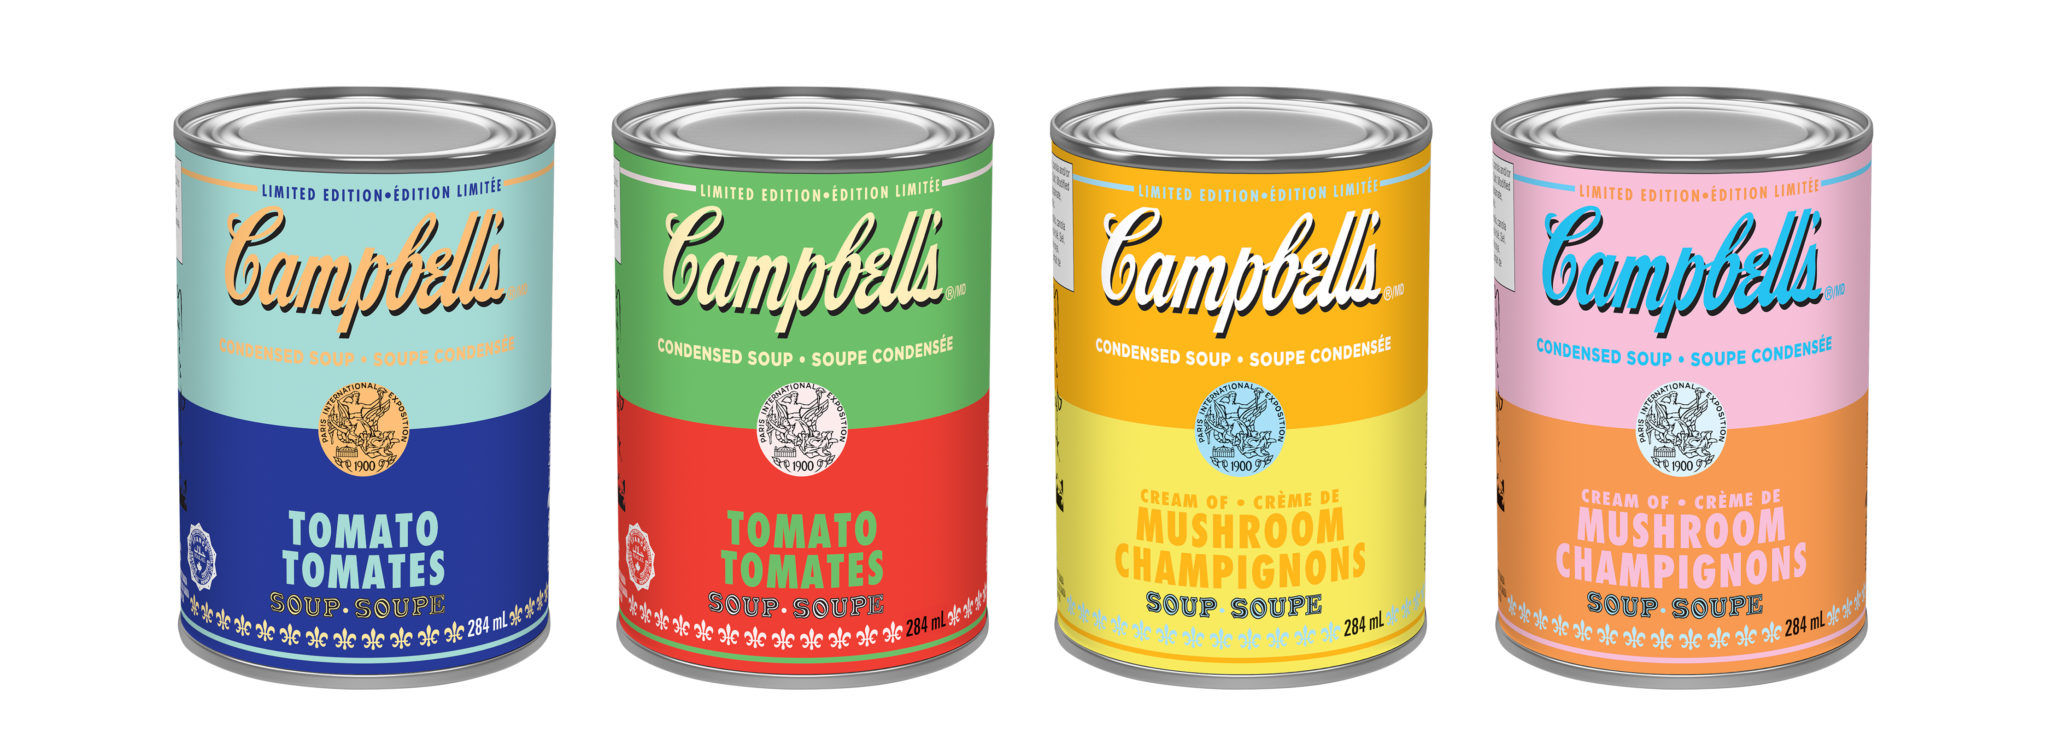
\includegraphics[width=10cm]{gfx/soupcans}
        \caption{Samenwerking van tooling binnen Eaglescience}
        \label{fig:es-tooling}
    \end{figure}

\end{itemize}


\section{Hoe wordt op dit moment software gedeployed?} \label{sec:hoe-wordt-op-dit-moment-software-gedeployed?}
Zoals hierboven is beschreven, wordt Jenkins gebruikt om de software te deployen. Het heeft de mogelijkheid om meerdere builds te doen voor verschillende projecten. Ieder project wordt op een eigen node gebouwd, waarbij de personal builds gehost worden op deze node. De development, en productie deploys gaan naar Azure in een specifiek ingerichte cluster voor deze omgevingen.

Een deploy wordt gedaan op het moment dat er source code naar GitLab gepushed wordt. Door middel van Tokens in de commit message kan gestuurd worden waar de build (als deze slaagt) gedeployed wordt bijv: {-all + portal} build en deployed alleen de portal. [ci-skip] zorgt ervoor dat er alleen een push wordt gedaan en geen build wordt gestart.
Samengevat worden er dus parameters meegegeven in de commit op basis waarvan wordt besloten of er een build moet plaatsvinden en zo ja waar en voor welke delen van de applicatie. Op deze manier wordt er flexibiliteit aan de ontwikkelaar geboden.

Een build en deploy gaat volgens de onderstaande afbeelding:

\begin{figure}[H]
    \myfloatalign
    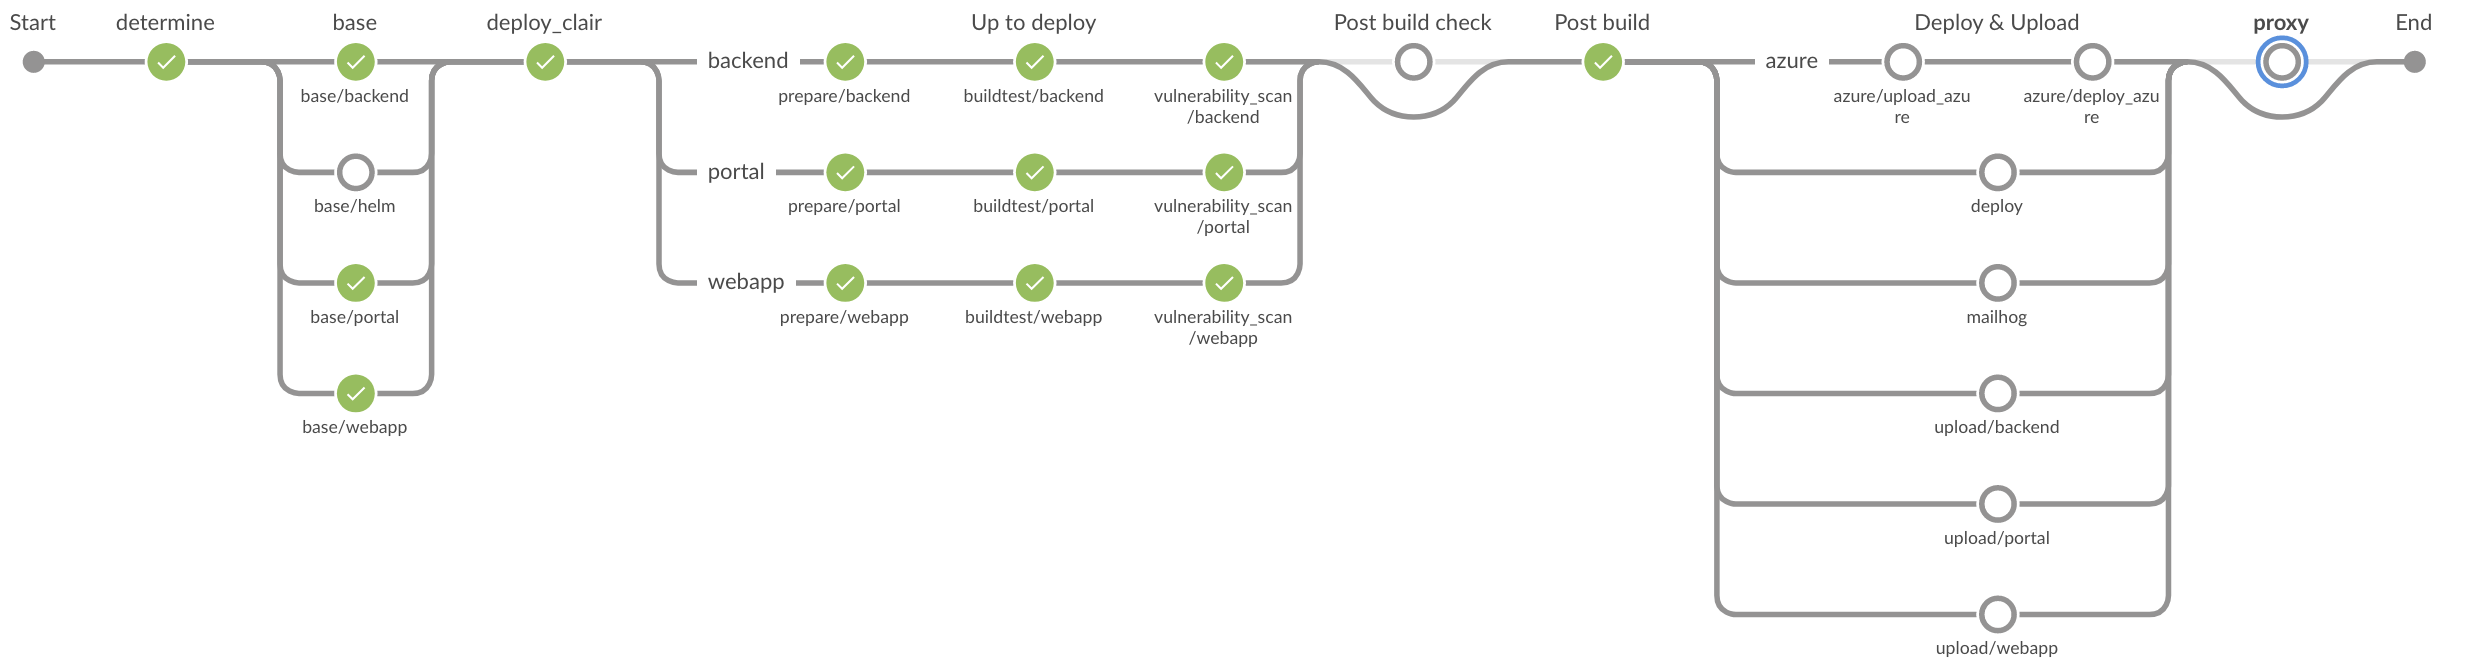
\includegraphics[width=15cm]{gfx/Screenshot 2021-08-18 Jenkins PipeLine}
    \caption{Jenkins(Blue Ocean) pipeline}
    \label{fig:JenkinsPipeLine}
\end{figure}
Een Jenkins pipeline werkt in een aantal stappen die in een .jenkinsFile worden beschreven, welke meegegeven wordt in een repository. Deze JenkinsFile wordt in de determine stap ingelezen waarna de benodigde stappen op een rij worden gezet. Hieronder worden deze stappen in meer detail beschreven:
\begin{itemize}
    \item \textbf{determine} Hier wordt bekeken,aan de hand van een JenkinsFile en tokens in de commit, welke stappen er nodig zijn om een succesvolle build en/of deploy te kunnen doen.
    \item \textbf{base} In de base stap worden alle Containers voorbereid die nodig zijn om de applicatie te builden. Images worden hier opgehaald waarna de containers worden voorbereid. De base stap is een parallel lopende stap waarin, in het voorbeeld van het figuur, backend, portal en de app worden voorbereid.
    \item \textbf{deploy clair} De clair scanner zoekt op kwetsbaarheden binnen containers die zojuist zijn aangemaakt. Dit is een extra veiligheid die ervoor zorgt dat de images en containers veilig zijn er alleen nog door bibliotheken die gebruikt worden voor ontwikkeling kwetsbaarheden kunnen worden toegevoegd.
    \item \textbf{Up to deploy}
    In het voorbeeld van het figuur wordt er voor de backend, portal, en app een parallel process gestart waarin de volgende drie substappen worden doorlopen:
    \begin{itemize}
        \item \textbf{prepare} Docker containers worden ingesteld en klaar gezet voor het ontvangen van de services.
        \item \textbf{builtest} De services worden gebuild en getest in deze stap. Eaglescience heeft een aantal tresholds opgesteld waaraan tests moeten voldoen. Om deze te analyseren worden de test resultaten vanuit de docker containers gekopieerd naar de Jenkins Store waar Jenkins de waarden kan analyseren. Als alle tests binnen de resultaten vallen wordt de volgende stap uitgevoerd.
        \item \textbf{vulnerability scan} Clair scanner scant nu de containers nogmaals, maar nu op de in de applicatie benodigde software (run time environments, databases etc.). Als clair iets vindt dat Eaglescience als verdacht acht dan wordt de build gestaakt.
    \end{itemize}
    \item \textbf{PostBuild(check)}
    Alle bevindingen worden hier gecheckt en mocht er iets mis zijn wordt er wederom afgebroken en is de build gefaald en zal er dus geen deploy plaatsvinden.
    \item \textbf{Deploy \& Upload}
    In het voorbeeld opgenomen in het figuur wordt de deploy niet uitgevoerd. Deze stap zorgt ervoor dat de gebouwde containers worden overgedragen naar Azure. Iedere container heeft wederom zijn eigen stappen. De upload valt echter buiten de scope van dit onderzoek.
    \item \textbf{End}
    Einde van de PipeLine Jenkins geeft de workers die het project heeft gebruikt weer vrij.
\end{itemize}


\section{Passende SCA tooling}\label{sec:sca-tooling}

In de opdracht staat vermeld dat de te ontwikkelen module eenvoudig in gebruik dient te kunnen worden genomen binnen de bestaande CI/CD Pipeline en dat de resultaten zichtbaar moeten zijn in de huidige portal. Hierom moet er dus Software Composition Analysis (SCA) tooling gevonden worden die makkelijk te integreren is in de huidige Jenkins pipeline, welke resultaten geeft die vervolgens te verwerken zijn tot een leesbare pagina in de portal. Als we deze stelling ontleden moeten er een aantal zaken worden onderzocht:
\begin{itemize}
    \item Welke tooling is er beschikbaar om SOUP-analyses uit te voeren op zowel SBT (Scala) als NPM (Node.js)-projecten?
    \item Welke resultaten worden er door de tool geproduceerd?
    \item Hoe kan de tooling worden geintegreerd in de huidige Jenkins pipeline?
\end{itemize}
Om deze vragen te beantwoorden moet er eerst geschikte tooling gevonden worden die, bij voorkeur, met zowel SBT als NPM-projecten overweg kan. Vervolgens dient er gekeken te worden naar hoe de geselecteerde tooling een resultaat bouwen, hoe deze eruit ziet en in welke tijd het resultaat gegeven kan worden.

\subsection{Tooling: Welke tooling is er beschikbaar om SOUP-analyses uit te voeren op zowel SBT (Scala) als NPM (Node.js)-projecten?}\label{subsec:ESTooling}
Er zijn een aantal bedrijven en instanties die tooling aanbieden om analyses te doen. Een google search op "Scala dependency scan" levert op de eerste resultaten pagina direct Snyk.io, SonarSource en OWASP op.

Snyk is een tool die geschikt is om Scala en TypeScript code, en dus bibliotheken te analyseren. Snyk kan worden ingezet op zowel SBT als NPM-projecten. Het biedt voor de analyse van code meerdere opties. Eén van die opties is middels een CLI Tool welke rapporteert naar een Dashboard gehost door Snyk zelf. Een andere optie die Snyk aanbiedt is te scannen middels een plugin via InteliJ, welke door Eaglescience gebruikt wordt. Als laatste optie biedt Snyk een plugin voor Jenkins die te integreren is in de buildstraat van Eaglescience. De voordelen van Snyk zijn dat er een volledig pakket wordt geboden, waarbij ook nog andere veiligheidsaspecten kunnen worden gecontroleerd (zoals het scannen van zelf geschreven code). Echter, om de volledige functionaliteit van Snyk te kunnen benutten is er een licentie nodig. Het nadeel hiervan is dat dit op periodieke basis geld kost. Een ander nadeel is dat de resulaten in een eigen omgeving, welke extern gehost wordt, kan worden ingezien. Hierdoor valt deze tooling echter buiten de vooraf gestelde criteria.

SonarSource is een ander bedrijf dat tooling aanbiedt voor het analyseren van source-code. Het doet dit door in de verschillende stadia van het proces tooling aan te bieden die helpen de kwaliteit van geleverde applicaties te verhogen. Als eerste biedt het een gratis plugin aan (SonarLint) voor verschillende IDE's waarbij actief wordt gekeken naar fouten, bugs en dergelijken tijdens het schrijven van code. Op die manier wordt er gekeken of code volgens standaarden worden geschreven en er geen kwetsbaarheden worden toegevoegd. Daarnaast is er een pakket dat SonarQube heet. Dit pakket biedt de mogelijkheid aan om op verschillende momenten naar de kwaliteit en de veiligheid van de aanwezige code te kijken. Hoewel SonarQube geschikt is om Scala en Typescript code te analyseren, is de SonarLint plugin niet compatibel met Scala code, maar wel met JavaScript en TypeScript. Er zijn meerdere versies beschikbaar die elk een specifiek aantal functionaliteiten aanbieden. Zo is er een community edition, welke gratis is, die als server geinstalleerd kan worden en waar verschillende repositories kunnen worden bijgehouden. Hiernaast zijn er andere editions beschikbaar waarvoor betaald moet worden en er extra functies worden geleverd, zoals GitLab integration en dergelijke. Samengevat zijn de voordelen van SonarSource tooling dat er tijdens alle stadia van software ontwikkeling controles worden ingebouwd die de code analyseren op o.a. kwetsbaarheden. Hiernaast kan SonarQube on premise draaien. Echter, een nadeel van de SonarQube plugin is dat SBT niet zelf door SonarSource ontwikkeld wordt, en SonarLint geen ondersteuning biedt voor SBT. De incompatibiliteit met Scala maakt integratie in de Eaglescience pipeline niet voor de hand liggend.

In eerdere onderzoeken is naar boven gekomen dat de OWASP zich bezig houd met het veilig houden van geschreven software. Een van de projecten die de OWASP aanbiedt is "Dependency-check". Dit is een Software Composition Analysis (SCA) Tool die het mogelijk maakt om openbaar gemaakte kwetsbaarheden te detecteren door te kijken of er voor dependencies een Common Platform Enumeration (CPE) bestaat. Als deze CPE bestaat kan er gekeken worden of er een CVE voor bestaat en vervolgens worden weergegeven in resultaten. Als geen van beiden bekend is wordt er door de tool vanuit gegaan dat er op het moment van checken geen kwetsbaarheid gevonden is. Hoewel dit op het oog een goede tool is om SOUP te analyseren, is de in het project ontwikkelde versie niet geschikt om te scannen op SBT en NPM dependencies. Op de website van het project is echter een link naar een versie die SBT-projecten kan analyseren. Uit de NPM repository blijkt dat er een soortgelijke tool bestaat om NPM-pakketten te analyseren.

De SBT depedency check en de OWASP dependency check (scanner voor NPM) lijken op dit moment de enige voor de hand liggende tooling voor de SOUP-analyse. Beide tooling zijn gratis beschikbaar en open-source. Echter zijn dit geen op zichzelf staande tools, maar bieden ze wel de mogelijkheid om te worden geintergreerd in suits zoals Snyk en SonarQube. Het feit dat ze losse tools zijn maakt het mogelijk om deze in te zetten in de buildstraat van Eaglescience. Een ander voordeel is dat beide tooling gebruik maken van dezelfde engine.


De tooling die geselecteerd zijn maken beide gebruik van de dependency-check engine uit het OWASP project.
De engine genereert een rapport door de beschreven dependencies te voorzien van een cpe(Common Platform enumeration). Deze CPE wordt vervolgens door de CVE database van het NIST gehaald. Als er zowel een CPE als een CVE gevonden wordt dan is er een kwetsbaarheid gevonden. Mocht een CPE missen dan gaat de tool ervan uit dat er geen kwetsbaaheid gevonden is. Om performance te verbeteren wordt er iedere 4 uur een update gehaald van de database en deze lokaal opgeslagen. Waarbij deze lokale database wordt gebruikt. na 4 uur wordt de database opnieuw geupdate om er op die manier voor te zorgen dat deze up to date is. Deze interval is in te stellen in de configuratie van de engine.

%
%https://github.com/etnetera/owasp-dependency-check for Node.js /NPM
%https://github.com/albuch/sbt-dependency-check for SBT
%
%https://github.com/eliasgranderubio/dagda niet zelfde als OWASP maar wellicht usefull

\subsection{Testen van Tools}\label{subsec:testen-van-tools}

Het lijkt voor de hand te liggen dat zowel de SBT-dependency-check en de OWASP-dependency-check (NPM) verantwoorde keuzes zijn om verder te onderzoeken. Echter dienen deze eerst te worden onderzocht op bruikbaarheid voordat er kan worden gedacht aan implementatie. Om de bruikbaarheid te testen zijn de volgende scenario's opgesteld die samen een idee moeten geven over de werking binnen een project en toepasbaarheid binnen een methode die in de volgende sectie zal worden onderzocht.

Er is gekozen voor twee scenario's
\begin{enumerate}
    \item \textbf{Bestaand Eaglescience Project} Om te achterhalen hoe de dependency check tools kunnen worden ingezet in projecten die op dit moment ontwikkeld en gehost worden, moeten de tools worden geintegreerd in een bestaand project. Als project is gekozen voor GroeiGids,\footnote{GroeiGids is op het moment van schrijven één van de grootste projecten waar Eaglescience aan werkt wanneer wordt gekeken naar code-volume en aantal depedencies. Het is een project in opdracht van de GGD en biedt ouders de mogelijkheid om groei informatie van hun kinderen in op te slaan.} een van de grotere projecten waar op dit moment aan wordt gewerkt. Het project bevat zowel een frontend (NPM Angular) als een App (NPM NativeScript), evenals een uit microservices bestaand SBT-project (geschreven in Scala) waarbij een andere manier wordt gebruikt om dependencies te declareren. Voor GroeiGids worden dependencies in een aparte file gedeclareerd en deze worden vervolgens geimporteerd in de build.sbt. Theoretisch gezien zou dit geen probleem moeten zijn gezien SBT zelf ook gebruik maakt van deze constructie.

    \item \textbf{Alleen de dependency declaraties} Door alleen dependency declaraties te gebruiken in een test, en dus niet het volledige project, kan worden onderzocht of de geselecteerde tooling hiermee om kan gaan. Dit zou wenselijk kunnen zijn om op een ander moment een analyse uit te voeren op de verschillende projecten. Het zou op die manier ook periodieke controle op kwetsbaarheden mogelijk maken zonder dat hiervoor een heel project opgezet dient te worden inclusief source-code.
\end{enumerate}

\subsubsection{Test 1a: SBT dependency scanning in een bestaand project}
\textbf{Doel:} Onderzoek naar het gebruik van de SBT-dependency-check plugin in GroeiGids. Het gewenste resultaat is kennis over hoe de plugin wordt geconfigureerd om de gewenste output, bij voorkeur een JSON file/object, te verkrijgen. Daarnaast wordt beoogd om inzicht te krijgen in hoeveel tijd de plugin nodig heeft voor het genereren van het rapport.
\textbf{Methode:} Als eerste dient de SBT-dependency-check plugin te worden geinstalleerd in het project middels de documentatie van het project. Vervolgens dient de output format te worden aangepast: \texttt{dependencyCheckFormats in Global += "JSON"}
en \texttt{dependencyCheckFormats in Global += "HTML"}. HTML wordt alleen gebruikt om in de test leesbare output te verkrijgen zodat deze kan worden geverifieerd met andere bronnen. Deze rapporten die resulteren in het draaien van \texttt{SBT dependencyCheck} dienen te worden gecontrolleerd tegen een andere bron. Daarnaast dient te worden bepaald hoeveel langer de analyse duurt wanneer de database wordt geupdate.
\textbf{Resultaat:} De analyse duurt ongeveer 173 seconden inclusief het ophalen/updaten van de database. Op het moment dat de database up-to-date is duurt een analyse 87 seconden. Dit zou dus inhouden dat een deploy 3 minuten langer duurt wanneer een SOUP-analyse wordt gedraaid voor een SBT project.
\begin{figure}[bth]
    \myfloatalign
    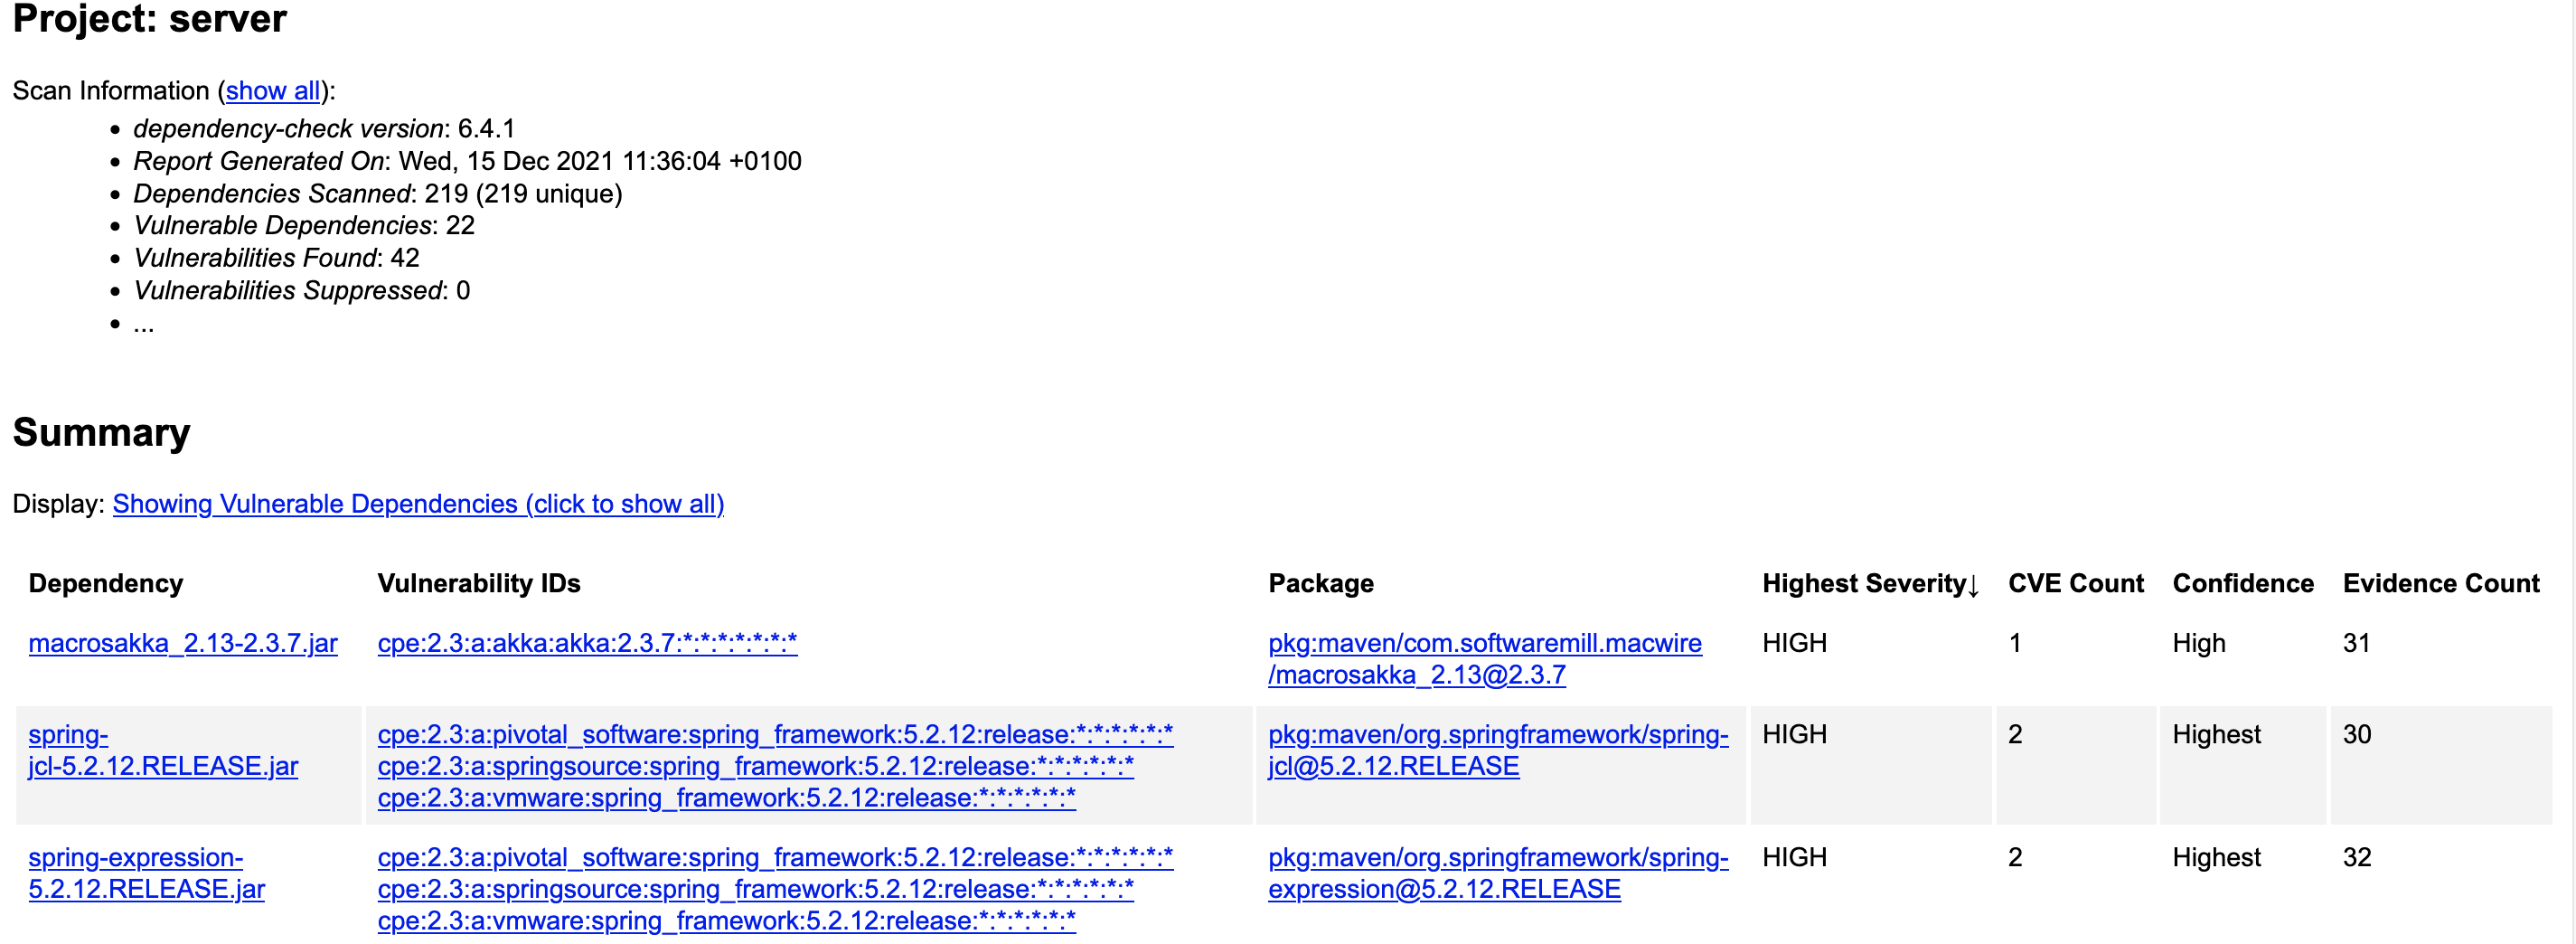
\includegraphics[width=15cm]{gfx/report_analyse_test1a_SBT}
    \caption{Deelresultaat van een analyse op de backend van GroeiGids}
    \label{fig:SBTReport1A}
\end{figure}

In figuur~\ref{fig:SBTReport1A} is te zien dat er 219 unieke dependencies gescanned zijn en dat er 42 kwetsbaarheden gevonden werden in 22 van de gescande dependencies. Na verificatie van de bovenste 5 vermeldingen tegen andere bronnen (opencve), bleek dat deze overeenkwamen, en het vertrouwen wordt daardoor gewekt dat de analyse correct is.

\subsubsection{Test 1b: NPM dependency scanning in een bestaand project}

\textbf{Doel:} Onderzoek naar de algemene werking van de geselecteerde plugin, waarbij vooral gekeken moet worden naar welke instellingen er relevant zijn en of de output nagenoeg overeenkomt met die van de SBT analyse. Daarnaast moet de timing worden opgenomen.
\textbf{Methode:} Voor NPM bestaat er geen plugin, welke wel beschikbaar is voor SBT-projecten. Echter kan de OWASP-dependency-check worden toegevoegd als een dev-dependency \texttt{npm install -D owasp-dependency-check}, waarna er een script moet worden aangemaakt in package.json die het volgende aanroept \texttt{"owasp-dependency-check --project \"GroeiGids APP\" -f JSON -f HTML -o \"./reports\""}. De tag HTML is hierin op genomen om de leesbaarheid te vergroten voor de peer-review.
\textbf{Resultaat:} De output van deze analyse is nagenoeg gelijk aan die van de hierboven uitgevoerde analyse op SBT. De output van de check ziet er qua opmaak hetzelfde uit als die van SBT. Ook de verificatie met OpenCVE is goed dus ook hier is er het vertrouwen dat de correcte resulaten worden weergeven. Daarnaast duurt de scan zonder update van de database 21 sec en 139 seconden met een update van een database, zie figuur~\ref{fig:NPMReport1b}.

\begin{figure}[bth]
    \myfloatalign
    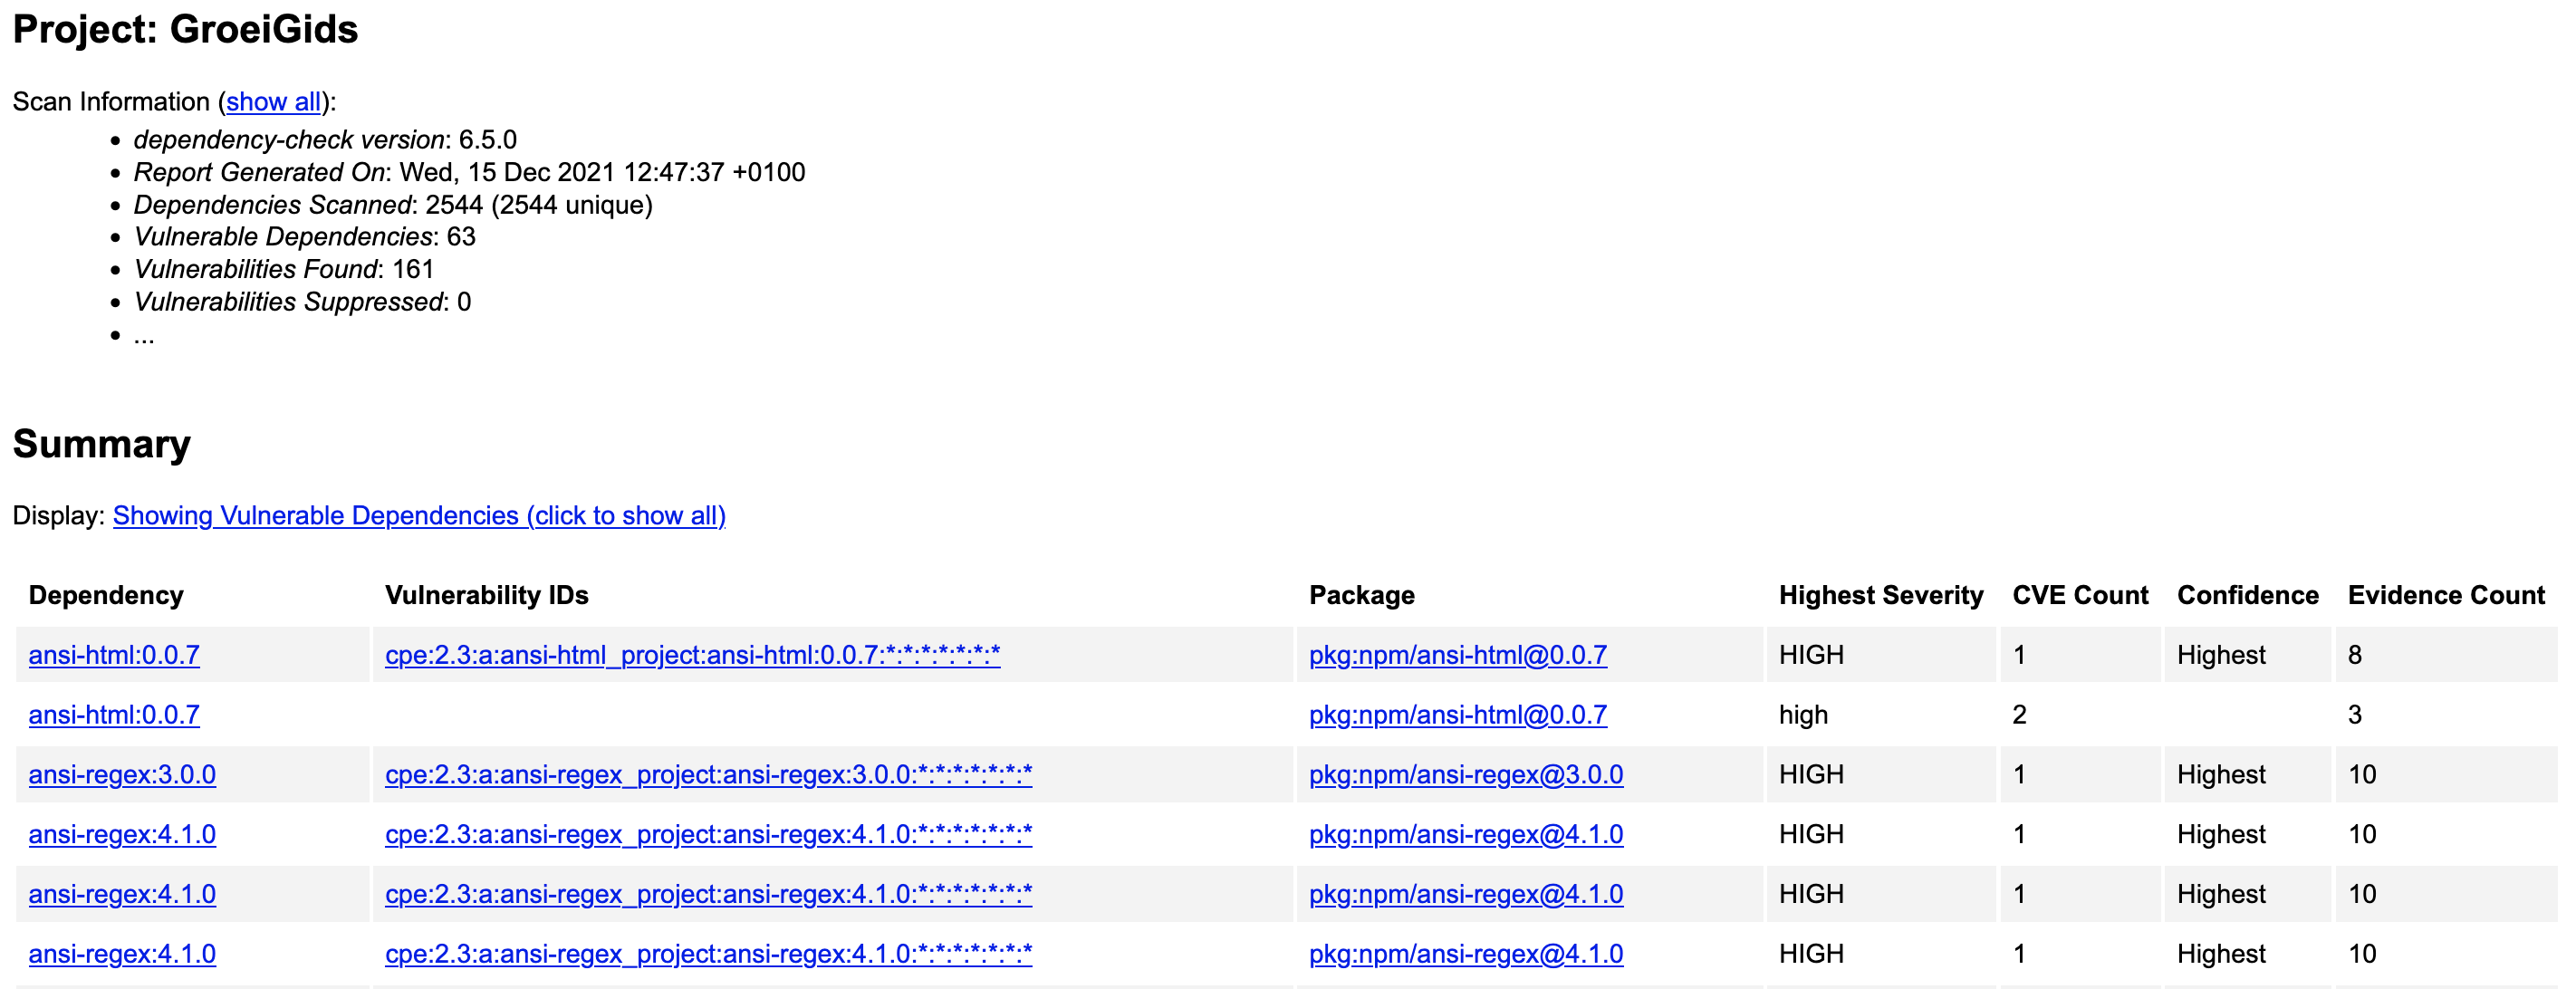
\includegraphics[width=15cm]{gfx/report_analyse_test1b_NPM}
    \caption{Deelresultaat van een analyse op de app van GroeiGids}
    \label{fig:NPMReport1b}
\end{figure}

Samengevat geven beide tools dezelfde rapporten comform hetzelfde JSON schema. Het feit dat deze overeenkomen biedt mogelijkheden voor het ontwikkelen van een enkele procedure voor het opnemen van deze rapporten in de API.
Wanneer de tijden van het scannen van de SBT en NPM bij elkaar worden opgeteld duurt de analyse 108 sec wanneer de database niet wordt geupdate. Wanneer dit wel het geval is duurt de test 208 sec.

\subsubsection{Test 2a: SBT alleen de dependency infomatie gebruiken}
Om te onderzoeken of een dependency check ook uitgevoerd kan worden zonder dat er een heel project bestaat en alleen een declaratie van dependencies in de build.sbt file staat wordt er een 2e test uitgevoerd.

\textbf{Doel:} Achterhalen welke bestanden er nodig zijn om een succesvolle analyse te doen. De uitkomsten moeten worden gecontroleerd op gelijkheid om te verifieren of deze methode dezelfde output genereeerd als in tests waarbij ook de source-code beschikbaar is.

[NOTE:] Checken waarom nu wel een aggregate functie moet worden toegepast.
%en 'dependencyCheck verandert in DependencyCheckAggregate.

\textbf{Methode:}Het GroeiGids project, welke gebruikt is voor de vorige test, wordt volledig gekopieerd naar een aparte folder, waarna alle source-code (incl. de bijbehorende mappen) wordt verwijderd. Het enige dat overblijft is de project folder mat daarin een plugins.sbt waar de dependencyCheck is gedefineerd, de dependencies.scala in de server folder en de build.sbt in de root. Vervolgens wordt de plugin gestart middels \textt{sbt dependencyCheckAggregate} en het resultaat in JSON vergeleken met het resultaat uit test 1a.

\textbf{Resultaat:} De rapporten die uitgegeven worden door zowel de eerste als de tweede test op het SBT project zijn gelijk. De scantijden zijn ongeveer hetzelfde, wat aangeeft dat deze methode van scannen een goed alternatief is voor het scannen van projecten, en ook gebruikt kan worden voor het periodiek scannen van een project. Van belang zijn de volgende bestanden: plugins.sbt, build.sbt en dependencies.scala omdat hier de dependency check plugin wordt gedefinieerd, als ook plugins benodigd voor het project. In build.sbt en dependencies.scala worden dependencies gedeclareerd.

%TODO naar resulaten sectie kijken

\subsubsection{Test 2b: NPM alleen de dependency infomatie gebruiken}
%Node.js docker container opzetten..
%package.json / package-lock.json copiere
%npm ci
%owasp script draaien
%cp resulst naar buiten
%destroy Container

Om te testen of de dependency check zonder informatie over het gebruik van de dependencies kan functioneren wordt er op een zelfde manier getest als bij test 2a, maar dan voor NPM projecten.

\textbf{Doel:}\\ Onderzoeken wat er nodig is om een dependency check uit te voeren zonder source-code. Het vermoeden bestaat dat package.json en package-lock.json voldoende informatie bevatten om dit volgens verwachting uit te voeren. Daarnaast moet er gekeken worden of de packages geinstalleerd dienen te worden.

\textbf{Methode:}
\texttt{NPM init} zal worden gebruikt om een nieuw leeg project op te zetten. Vervolgens moeten de dependency declaraties worden gekopieerd; package.json en package-lock.json.

Hierna wordt de dependency check toegevoegd aan package.json middels \texttt{npm -D install owasp-dependency-check}. Hierna moet er een \texttt{NPM ci} worden uitgevoerd om de declaraties in package-lock.json te installeren. Dit resulteerd in een project zonder source-code, maar met geinstalleerde dependencies zoals ze het laatst bekend waren (bijv tijdens deploy).

Vervolgens kan er middels een in package.json gedefineerd script: \texttt{"owasp": "owasp-dependency-check --project \" angularSandbox \" -f JSON -l\"dep-check-log.txt\" "}%TODO quotes goedzetten
een rapport worden gegeneerd, dat vergeleken kan worden met de uitkomsten van test 1b.

\textbf{Resultaat:}\\
Er kan enkel een analyse gedaan worden op het moment dat er zowel een package.json bestaat (declaratie van het script) als een package-lock.json (feitelijke dependency definitie van een laatste install), Daarnaast dienen ook de dependencies te zijn geinstalleerd. Kennelijk is dit een vereiste vanuit de OWASP dependency check. In de logs zijn ook statements te vinden die erop wijzen dat niet geinstalleerde dependencies worden geskipped
\texttt{2021-12-13 15:08:36,500 org.owasp.dependencycheck.analyzer.NodePackageAnalyzer:292
WARN  - dependency skipped: node module esbuild-darwin-arm64 seems optional and not installed}.

%De NPM Dependency check voert onderwater het volgende commando uit \texttt{/dependency-check.sh --out=./dependency-check-reports --project angularSandbox -f JSON --data=/tmp/dependency-check-data --scan=package-lock.json
%} de -f en de --out flags zijn de output flags die aangeven dat er een JSON file in depende-check-reports directory in de base gemaakt moet worden. --scan = package-lock.json is het bestand wat geacanned wordt wat wil zeggen dat er een node_modules folder moet zijn is aangemaakt middels een npm install op de package.json van het project.

\subsubsection{Conclusie tests}
Een analyse voor een project zo groot als GroeiGids duurt in het slechtste geval ongeveer 4 minuten. Hierbij is geen rekening gehouden met andere taken die processor tijd vragen. Deze tijd zal oplopen op het moment dat de Jenkins Server meerdere builds aan het uitvoeren is voor meerdere projecten. Echter zijn de rapporten in zowel test 1 als test 2 gelijk dus kunnen we beide manieren gebruiken voor de ontwikkeling van een methode.


\newpage
\section{Methode voor extractie, verwerken en het publiceren van de resultaten gevonden in de projecten van Eaglescience}\label{subsec:methodeSOUPES}

Er moet een methode worden ontwikkeld die in staat is om door de buildstraat gegenereerde gegevens te gebruiken voor het opbouwen van een rapport die in de portal te lezen is.
Deze methode moet op twee manieren werken:
Ten eerste moet het een dependency check uitvoeren tijdens het uitrollen om een rapport aan te kunnen bieden op het moment van deploy in Azure. Daarnaast moet het ook gegevens over het project zoals de dependecy declaraties, project en build meta klaarzetten in een scan que, zodat hiervan op een later moment gebruik van kan worden gemaakt.

De details van deze methode worden hieronder beschreven.

\begin{figure}
    \centering
    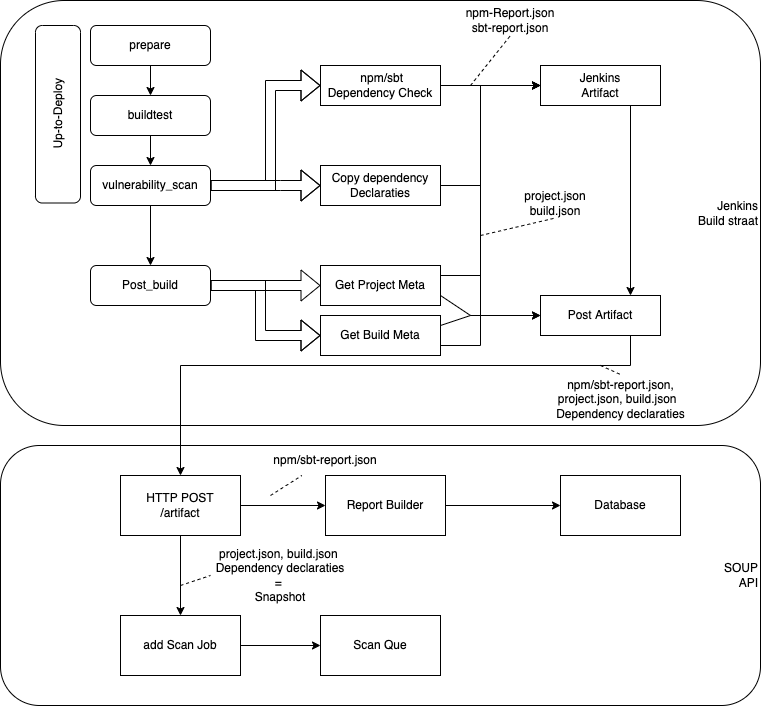
\includegraphics[width=15cm]{gfx/methode_Jenkins}
    \caption{Methode SOUP analyse}
    \label{fig:methodeSOUPanalyse}
\end{figure}

In figuur~\ref{fig:methodeSOUPanalyse} is de methode voor de SOUP analyse uitgewerkt voor NPM en SBT. Voor beiden gelden globaal dezelfde stappen. Er zijn twee momenten waarop nuttige informatie kan worden verkregen uit de pipeline wanneer hieraan functionaliteiten worden toegevoegd ten behoeve van SOUP analyse. Ten eerste is dit de \texttt{Vulnerability\_scan} stap, en ten tweede de \texttt{post\_build} stap. In de \texttt{Vulnerability\_scan} stap is de module gereed en kan deze gescaned worden op vulnerabilities. Door hieraan de dependency check toe te voegen kan er een rapport gegenereerd worden die in de Jenkins artifacts wordt opgeslagen. In deze stap wordt in dezelfde Jenkins artifacts ook de dependency declaraties opgeslagen voor dezelfde module.

Op dit moment is bekend welke dependencies er gebruikt worden en is er een check uitgevoerd. Om erachter te komen voor welk project dit is dient er in de post build stap metadata toegevoegd te worden die helpen bij de indentificatie van het project. De project metadata omvat o.a. project naam, URL repo en welke modules het project bevat. De build metadata bevat o.a. de timestamp van de build, het resultaat van de build en welke githash er gebuild is. Deze metadata wordt ook in de Jenkins artifacts opgeslagen. Daarna worden alle artifacts gepost naar de SOUP API.
De SOUP API haalt hieruit de SBT (sbt-report.json) en NPM (npm-report.json) rapporten gegenereerd door de dependency check. Vervolgens worden hieruit de relevante data gefilterd door de report builder, welke het daarop in een database plaatst die door de portal gebruikt kan worden.


Om periodiek te kunnen scannen, worden de project en build metadata samen met de dependency declaraties als een snapshot in een scan que gezet. Deze scan que kan periodiek worden doorlopen, om de projecten die hierin staan te scannen op kwetsbaarheden waarvoor de dependency check gebruikt wordt. Via de report builder zullen hiervan de resultaten in de database worden geplaatst.

\subsection{Resultaat}
Door in de buildstraat te scannen wordt er een rapport ten tijde van de build gegenereerd. Ondanks dat dit de duur van de deploy kan verlengen wordt er hierdoor gegarandeerd dat er een rapport beschikbaar is over de uitgerolde externe bibliotheken. Door in dezelfde stap ook alle in het project aanwezige declaraties beschikbaar te stellen voor de SOUP API kan er op basis van die declaraties periodiek een analyse worden uitgevoerd. Door zowel de resultaten van de dependency check als de dependency declaraties waar deze check op is uitgevoerd veilig te stellen weet je zeker dat de periodieke scans dezelfde basis hebben als de tijdens de deploy uitgevoerde scan. De methode voor het periodiek scannen geeft de mogelijkheid om te scannen tijdens voor de server rustige momenten. Hierdoor is er minder impact van de SOUP analyse op de performance tijdens kantooruren.

\subsection{Conclusie}\label{sec:conclusie}
De hierboven genoemde methode maakt het in theorie mogelijk om middels een depedency check geautomatiseerd een SOUP analyse uit te voeren tijdens de uitrol van een project, met als resultaat een rapport over de eventueel gevonden kwetsbaarheden. Tijdens de methode worden de projectgegevens veilig gesteld waardoor later op periodieke basis dezelfde dependency check kan worden uitgevoerd.
Deze methode maakt het mogelijk om inzichten te krijgen zodat de preventie stappen beschreven in OWASP top 10 - A06:2021 "Vulnerable and outdated components" kunnen worden nageleefd.


\section{Eindconclusie}\label{sec:Eindconclusie}
In dit hoofdstuk zijn een aantal onderzoeken uitgevoerd. Deze hebben inzichten opgeleverd over hoe Eaglescience software ontwikkeld, waarbij aandacht is besteed aan de devstack, werkwijze en tooling. Deze bevindingen vormden de basis voor de zoektocht naar compatibele tooling voor SOUP analyses binnen Scala en TypeScript projecten, waarbij SBT en NPM worden gebruikt als buildtools. Doordat Eaglescience ontwikkeld in een 'niche-taal' (Scala) is de beschikbare tooling gelimiteerd. Desondanks is er voor beide door Eaglescience gebruikte hoofdtalen geschikte tooling gevonden om SOUP analyses mee uit te voeren (OWASP-dependency-check voor NPM en sbt-dependency-check voor SBT). Uit documentatie van deze tooling bleek dat er testen mee konden worden uitgevoerd om te onderzoeken hoe ze in een methode zouden kunnen worden geimplementeerd om aan de project eisen te kunnen voldoen. De geselecteerde tooling bleken compatibel en goed te werken tijdens een reeks testen, en te voldoen aan de in de opdracht gestelde eisen. Tijdens deze testen werd inspiratie opgedaan voor een methode om gegevens uit de Jenskins buildstraat te verkrijgen en te analyseren. Door samenvoeging van de twee testmethodes is er een methode gevonden voor de analyse van externe bibliotheken binnen Eaglescience projecten. Deze methode maakt het in theorie mogelijk om zowel na deploy geautomatiseerd te draaien als op periodieke basis. De bevindingen van dit hoofdstuk zullen als basis dienen voor het ontwerp van de daadwerkelijke module voor de uitvoering van SOUP analyses.



%De twee tools draaien beiden op de zelfde engine. wat er vervolgens voor zorgt dat er voor beide tools nagenoeg de zelfde output is. Echter door de complexiteit van de projecten die uitgerold worden is voor de SBT tool veel werk om alle dependencie te analyseren wat niet te goed komt in de build tijd. op basis van dit gegeven is er voor gekozen om later een analyse uit te voeren op de dependencies en de pipeline alleen de gebruikte dependencies en hun versies te borgen in een snapshot in de database en deze snapshots periodiek te analyseren op kwetsbaarheden. Het voordeel van deze manier is naast dat het minder tijd kost in de build pipeline. we de analyse kunnen uitvoeren op ieder gewenst moment en dus ook in de nachtelijke uren wanneer de servers niet de druk hebben die ze overdag hebben. Voor het ontwerp moet er dan ook een manier gevonden worden om snapshots op te slaan waarin minimaal de volgende attributen zijn vastgelegd:

%Kan er worden achterhaald door middel van ene Hash of de commit nieuwer is?
%Voorhet maken van de snapshots moeten er in de jenkins pipeline een mechaniek worden geplaatst die de gevonden attributen kan opslaan in een database voor later gebruik.
%Een bijkomend voordeel van deze manier van werken is dat er een historiek onstaat in de gebruikte versies welke als bewijsvoering kan dienen bij incidenten.

%\subsection{Methode 1: Scannen in de buildstraat}
%In de jenkinsFile voor de stap(vulnerability\_scan) moet een task worden toegevoegd die anvullende taken uitvoerd voor zowel de backend als frontend modules. Beide zijn verschillende en worden dan ook apart beschreven waarbij er van uitgegaan wordt dat tijdens de laatste commit de benodigde tooling is declareerd in de modules dus (sbt-dependency-check plug-in in de plugins.sbt, en owasp-dependency-check als dev-dependency met executor script) Op dit moment van de pipeline zijn er images beschikbaar waarvan containers gestart kunnen worden. Naast het rapport voor iedere module dient er ook meta data van het project als ook van de scan worden opgeslagen
%
%\textbf{Frontend} De volgende stappen moeten worden uitgevoerd om een volledige JSON rapport te versturen vanuit een NPM project naar de SOUPAPI.
%\begin{enumerate}
%    \item Genereren van een SOUP rapport voor de module.
%    \begin{enumerate}
%        \item Opstarten van de contriner die gebuild is tijdens de build/test stap
%        \item \texttt{npm run owasp} draaien voor het genereneren van het rapport.
%        \item Rapport copieren naar de Jenkins Artifact store.
%        \item Optioneel checken naar threshold
%    \end{enumerate}
%\end{enumerate}
%
%\textbf{Backend} Feitelijk worden dezelfde stappen uitgevoerd voor de backend als voor de frontend. met als grote verschil de SBT plugin in plaats van de npm run aanroep. Het resultaat is eveneens een JSON rapport.
%\begin{enumerate}
%    \item Genereren van een SOUP rapport voor de module.
%    \begin{enumerate}
%        \item Opstarten van de contriner die gebuild is tijdens de build/test stap
%        \item \texttt{sbt dependenceCheckAggregate} draaien voor het genereneren van het rapport.
%        \item Rapport copieren naar de Jenkins Artifact store.
%        \item Optioneel checken naar threshold
%    \end{enumerate}
%\end{enumerate}
%
%Vervolgens moet er in de \text{post\_build} stap een aantal gegevens worden verzameld die nodig zijn voor de identifictie van de scan. Als ook de rapporten zelf.
%\begin{itemize}
%    \item Project naame
%    \item Timestamp build
%    \item project type(SBT/NPM)
%    \item Hash van de commit die de build heeft getriggered
%    \item Buildtool Version
%    \item runtime Version
%    \item Build target (development, Acceptance, Productie)
%    \item Build status (OK, FAIL)
%\end{itemize}
%Aan dit rijtje worden dus de twee JSON bestanden toegevoegd en deze worden middels een HTTP POST method geupload naar de SOUPAPI waar deze vervolgens verder wordt verwerkt tot een voor de portal bruikbare bron.
%
%
%\begin{figure}[bth]
%    \myfloatalign
%    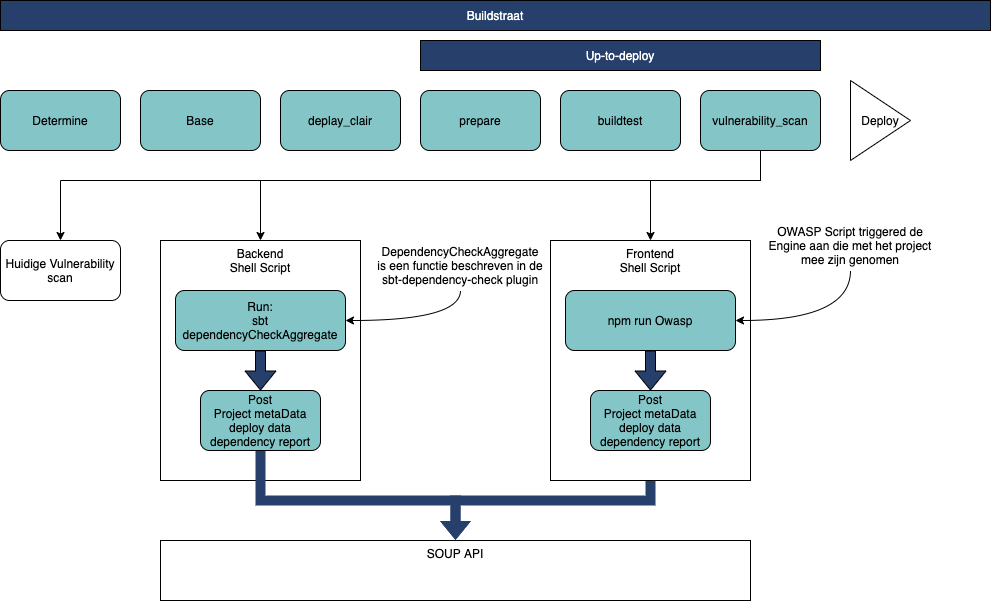
\includegraphics[width=10cm]{gfx/Methode_1}
%    \caption{Methode 1 schema}
%    \label{fig:methode1Schema}
%\end{figure}
%
%\begin{enumerate}
%    \item
%\end{enumerate}
%\begin{itemize}
%    \item Voordelen   \begin{itemize}
%                          \item Bij iedere deploy naar een ingesteld omgeving is er een snapshot van de gebruikte bibliotheken
%                          \item Er is een mogelijkheid om de build te stoppen op het moment dat de threshold van toelaatbare kwetsbaarheden wordt overschreden.
%    \end{itemize}
%    \item Nadelen  \begin{itemize}
%                       \item Bij een periodieke check moet er een nieuwe build worden gestart wat weer tot onnodig verbruik van resources leidt.
%                       \item
%    \end{itemize}
%\end{itemize}
%
%\subsection{Methode 2: postponed analyseren}
%Scannen op een later moment, dus door een project te bouwen op basis van een snapshot en deze op een later moment te analyseren.
%In de JenkinsFile voor de stap moet er voor de post\_build stap een task worden toegevoegd die anvullende taken voor het opslaan van project metadata, build metadata de data over de commit die gebuild is. Daarnaast worden de bestanden waarin informatie over de gebruikte dependencies ook meegestuurd zodat er op een later moment een project van kan worden gebouwd zoals gedemonstreerdt in test 2.
%De volgende attributen zijn nodig om een build te identificeren en opnieuw op een andere plaats te verbouwen.
%\begin{itemize}
%    \item Project naame
%    \item Timestamp build
%    \item project type(SBT/NPM)
%    \item Hash van de commit die de build heeft getriggered
%    \item Buildtool Version
%    \item runtime Version
%    \item Build target (development, Acceptance, Productie)
%    \item Build status (OK, FAIL)
%    \item Bestanden uit portal: package.json , Package-lock.json
%    \item Bestanden uit App: Package.json, Package-lock.json
%    \item Bestanden uit SBT: build.sbt, dependencies.scala en de plugin.sbt.
%\end{itemize}
%Door deze attributen in een snapshot op te slaan in een database kan er op een later moment een analyse worden uitgevoerd.
%
%\begin{figure}[bth]
%    \myfloatalign
%    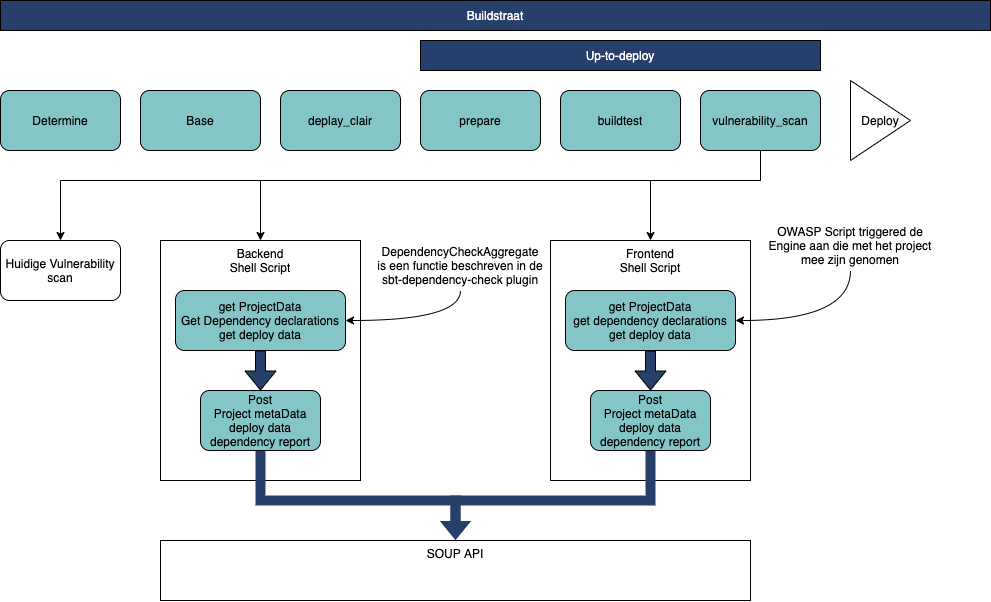
\includegraphics[width=15cm]{gfx/Methode_2}
%    \caption{Methode 2 schema}
%    \label{fig:methode2Schema}
%\end{figure}


%Binnen EagleScience wordt er gewerkt middels de SCRUM methode om software te ontwikkelen. Waarbij Jira en Confluence worden gebruikt voor de documentatie van de projecten. Het zou voor de hand kunnen liggen om informatie over de SOUP analyses in Confluence op te slaan zodat er mee gelift kan worden op dit systeem. Echter doordat de end of life van Confluence is aangekondigd dient er een alternatief worden gezocht. Welke al in de opdracht is meegenomen.



%\part{Implementatie}\label{prt:Implementatie}


\cleardoublepage % Empty page before the start of the next part

%----------------------------------------------------------------------------------------
%	THESIS CONTENT - APPENDICES
%----------------------------------------------------------------------------------------

\appendix

\part{Appendix} % New part of the thesis for the appendix

% Appendix A

\chapter{Appendix Test}

%----------------------------------------------------------------------------------------

\lipsum[13-14]

%----------------------------------------------------------------------------------------

\section{Appendix Section Test}
\lipsum[15]

\graffito{More dummy text}
\lipsum[16]

%----------------------------------------------------------------------------------------

\section{Another Appendix Section Test}
\lipsum[17]

\begin{table}
\myfloatalign
\begin{tabularx}{\textwidth}{Xll} \toprule
\tableheadline{labitur bonorum pri no} & \tableheadline{que vista}
& \tableheadline{human} \\ \midrule
fastidii ea ius & germano &  demonstratea \\
suscipit instructior & titulo & personas \\
\midrule
quaestio philosophia & facto & demonstrated \\
\bottomrule
\end{tabularx}
\caption[Autem usu id]{Autem usu id.}
\label{tab:moreexample}
\end{table}

\lipsum[18]

There is also a useless Pascal listing below: \autoref{lst:useless}.

\begin{lstlisting}[float=b,language=Pascal,frame=tb,caption={A floating example (\texttt{listings} manual)},label=lst:useless]
for i:=maxint downto 0 do
begin
{ do nothing }
end;
\end{lstlisting} % Appendix A
%% Appendix X

\chapter{Appendix Title}

%----------------------------------------------------------------------------------------

% Content begins here % Appendix B - empty template

%----------------------------------------------------------------------------------------
%	POST-CONTENT THESIS PAGES
%----------------------------------------------------------------------------------------

\cleardoublepage% Bibliography

\label{app:bibliography} % Reference the bibliography elsewhere with \autoref{app:bibliography}

\manualmark % Work-around to have small caps also here in the headline
\markboth{\spacedlowsmallcaps{\bibname}}{\spacedlowsmallcaps{\bibname}} % Work-around to have small caps also
%\phantomsection
\refstepcounter{dummy}

\addtocontents{toc}{\protect\vspace{\beforebibskip}} % Place the bibliography slightly below the rest of the document content in the table of contents
\addcontentsline{toc}{chapter}{\tocEntry{\bibname}}


\printbibliography
 % Bibliography

\cleardoublepage% Declaration

\refstepcounter{dummy}
\pdfbookmark[0]{Declaration}{declaration} % Bookmark name visible in a PDF viewer

\chapter*{Declaration} % Declaration section text

\thispagestyle{empty}

Put your declaration here.
\bigskip
 
\noindent\textit{\myLocation, \myTime}

\smallskip

\begin{flushright}
\begin{tabular}{m{5cm}}
\\ \hline
\centering\myName \\
\end{tabular}
\end{flushright}
 % Declaration

\cleardoublepage% Colophon (a brief description of publication or production notes relevant to the edition)

\pagestyle{empty}

\hfill

\vfill

\pdfbookmark[0]{Colophon}{colophon}

\section*{Colophon}

This document was typeset using the typographical look-and-feel \texttt{classicthesis} developed by Andr\'e Miede. The style was inspired by Robert Bringhurst's seminal book on typography ``\emph{The Elements of Typographic Style}''. \texttt{classicthesis} is available for both \LaTeX\ and \mLyX: 

\begin{center}
\url{https://bitbucket.org/amiede/classicthesis/}
\end{center}

\noindent Happy users of \texttt{classicthesis} usually send a real postcard to the author, a collection of postcards received so far is featured here: 

\begin{center}
\url{http://postcards.miede.de/}
\end{center}
 
\bigskip

\noindent\finalVersionString % Colophon

%----------------------------------------------------------------------------------------

\end{document}
